% Options for packages loaded elsewhere
\PassOptionsToPackage{unicode}{hyperref}
\PassOptionsToPackage{hyphens}{url}
%
\documentclass[
]{book}
\usepackage{amsmath,amssymb}
\usepackage{iftex}
\ifPDFTeX
  \usepackage[T1]{fontenc}
  \usepackage[utf8]{inputenc}
  \usepackage{textcomp} % provide euro and other symbols
\else % if luatex or xetex
  \usepackage{unicode-math} % this also loads fontspec
  \defaultfontfeatures{Scale=MatchLowercase}
  \defaultfontfeatures[\rmfamily]{Ligatures=TeX,Scale=1}
\fi
\usepackage{lmodern}
\ifPDFTeX\else
  % xetex/luatex font selection
\fi
% Use upquote if available, for straight quotes in verbatim environments
\IfFileExists{upquote.sty}{\usepackage{upquote}}{}
\IfFileExists{microtype.sty}{% use microtype if available
  \usepackage[]{microtype}
  \UseMicrotypeSet[protrusion]{basicmath} % disable protrusion for tt fonts
}{}
\makeatletter
\@ifundefined{KOMAClassName}{% if non-KOMA class
  \IfFileExists{parskip.sty}{%
    \usepackage{parskip}
  }{% else
    \setlength{\parindent}{0pt}
    \setlength{\parskip}{6pt plus 2pt minus 1pt}}
}{% if KOMA class
  \KOMAoptions{parskip=half}}
\makeatother
\usepackage{xcolor}
\usepackage{color}
\usepackage{fancyvrb}
\newcommand{\VerbBar}{|}
\newcommand{\VERB}{\Verb[commandchars=\\\{\}]}
\DefineVerbatimEnvironment{Highlighting}{Verbatim}{commandchars=\\\{\}}
% Add ',fontsize=\small' for more characters per line
\usepackage{framed}
\definecolor{shadecolor}{RGB}{248,248,248}
\newenvironment{Shaded}{\begin{snugshade}}{\end{snugshade}}
\newcommand{\AlertTok}[1]{\textcolor[rgb]{0.94,0.16,0.16}{#1}}
\newcommand{\AnnotationTok}[1]{\textcolor[rgb]{0.56,0.35,0.01}{\textbf{\textit{#1}}}}
\newcommand{\AttributeTok}[1]{\textcolor[rgb]{0.13,0.29,0.53}{#1}}
\newcommand{\BaseNTok}[1]{\textcolor[rgb]{0.00,0.00,0.81}{#1}}
\newcommand{\BuiltInTok}[1]{#1}
\newcommand{\CharTok}[1]{\textcolor[rgb]{0.31,0.60,0.02}{#1}}
\newcommand{\CommentTok}[1]{\textcolor[rgb]{0.56,0.35,0.01}{\textit{#1}}}
\newcommand{\CommentVarTok}[1]{\textcolor[rgb]{0.56,0.35,0.01}{\textbf{\textit{#1}}}}
\newcommand{\ConstantTok}[1]{\textcolor[rgb]{0.56,0.35,0.01}{#1}}
\newcommand{\ControlFlowTok}[1]{\textcolor[rgb]{0.13,0.29,0.53}{\textbf{#1}}}
\newcommand{\DataTypeTok}[1]{\textcolor[rgb]{0.13,0.29,0.53}{#1}}
\newcommand{\DecValTok}[1]{\textcolor[rgb]{0.00,0.00,0.81}{#1}}
\newcommand{\DocumentationTok}[1]{\textcolor[rgb]{0.56,0.35,0.01}{\textbf{\textit{#1}}}}
\newcommand{\ErrorTok}[1]{\textcolor[rgb]{0.64,0.00,0.00}{\textbf{#1}}}
\newcommand{\ExtensionTok}[1]{#1}
\newcommand{\FloatTok}[1]{\textcolor[rgb]{0.00,0.00,0.81}{#1}}
\newcommand{\FunctionTok}[1]{\textcolor[rgb]{0.13,0.29,0.53}{\textbf{#1}}}
\newcommand{\ImportTok}[1]{#1}
\newcommand{\InformationTok}[1]{\textcolor[rgb]{0.56,0.35,0.01}{\textbf{\textit{#1}}}}
\newcommand{\KeywordTok}[1]{\textcolor[rgb]{0.13,0.29,0.53}{\textbf{#1}}}
\newcommand{\NormalTok}[1]{#1}
\newcommand{\OperatorTok}[1]{\textcolor[rgb]{0.81,0.36,0.00}{\textbf{#1}}}
\newcommand{\OtherTok}[1]{\textcolor[rgb]{0.56,0.35,0.01}{#1}}
\newcommand{\PreprocessorTok}[1]{\textcolor[rgb]{0.56,0.35,0.01}{\textit{#1}}}
\newcommand{\RegionMarkerTok}[1]{#1}
\newcommand{\SpecialCharTok}[1]{\textcolor[rgb]{0.81,0.36,0.00}{\textbf{#1}}}
\newcommand{\SpecialStringTok}[1]{\textcolor[rgb]{0.31,0.60,0.02}{#1}}
\newcommand{\StringTok}[1]{\textcolor[rgb]{0.31,0.60,0.02}{#1}}
\newcommand{\VariableTok}[1]{\textcolor[rgb]{0.00,0.00,0.00}{#1}}
\newcommand{\VerbatimStringTok}[1]{\textcolor[rgb]{0.31,0.60,0.02}{#1}}
\newcommand{\WarningTok}[1]{\textcolor[rgb]{0.56,0.35,0.01}{\textbf{\textit{#1}}}}
\usepackage{longtable,booktabs,array}
\usepackage{calc} % for calculating minipage widths
% Correct order of tables after \paragraph or \subparagraph
\usepackage{etoolbox}
\makeatletter
\patchcmd\longtable{\par}{\if@noskipsec\mbox{}\fi\par}{}{}
\makeatother
% Allow footnotes in longtable head/foot
\IfFileExists{footnotehyper.sty}{\usepackage{footnotehyper}}{\usepackage{footnote}}
\makesavenoteenv{longtable}
\usepackage{graphicx}
\makeatletter
\def\maxwidth{\ifdim\Gin@nat@width>\linewidth\linewidth\else\Gin@nat@width\fi}
\def\maxheight{\ifdim\Gin@nat@height>\textheight\textheight\else\Gin@nat@height\fi}
\makeatother
% Scale images if necessary, so that they will not overflow the page
% margins by default, and it is still possible to overwrite the defaults
% using explicit options in \includegraphics[width, height, ...]{}
\setkeys{Gin}{width=\maxwidth,height=\maxheight,keepaspectratio}
% Set default figure placement to htbp
\makeatletter
\def\fps@figure{htbp}
\makeatother
\setlength{\emergencystretch}{3em} % prevent overfull lines
\providecommand{\tightlist}{%
  \setlength{\itemsep}{0pt}\setlength{\parskip}{0pt}}
\setcounter{secnumdepth}{5}
\usepackage{booktabs}

\usepackage{color}
\usepackage{framed}
\setlength{\fboxsep}{.8em}

% These colours were manually entered, they shouldn't matter unless you want pdf output

\newenvironment{redbox}{
  \definecolor{shadecolor}{RGB}{243, 154, 157}
  \color{white}
  \begin{shaded}}
 {\end{shaded}}

\newenvironment{bluebox}{
  \definecolor{shadecolor}{RGB}{172, 210, 237}
  \color{white}
  \begin{shaded}}
 {\end{shaded}}

\newenvironment{greenbox}{
  \definecolor{shadecolor}{RGB}{141, 181, 128}
  \color{white}
  \begin{shaded}}
 {\end{shaded}}
\ifLuaTeX
  \usepackage{selnolig}  % disable illegal ligatures
\fi
\usepackage[]{natbib}
\bibliographystyle{plainnat}
\usepackage{bookmark}
\IfFileExists{xurl.sty}{\usepackage{xurl}}{} % add URL line breaks if available
\urlstyle{same}
\hypersetup{
  pdftitle={Analysis Using R 2024},
  pdfauthor={Faculty: Shraddha Pai, Chaitra Sarathy, Ian Cheong, Zoe Klein, Amin Nooranikhojasteh, Nia Hughes},
  hidelinks,
  pdfcreator={LaTeX via pandoc}}

\title{Analysis Using R 2024}
\author{Faculty: Shraddha Pai, Chaitra Sarathy, Ian Cheong, Zoe Klein, Amin Nooranikhojasteh, Nia Hughes}
\date{June 13, 2024 - June 14, 2024}

\begin{document}
\maketitle

{
\setcounter{tocdepth}{1}
\tableofcontents
}
\part{Introduction}\label{part-introduction}

\chapter{Workshop Info}\label{workshop-info}

Welcome to the 2024 Analysis Using R Canadian Bioinformatics Workshop webpage!

\section{Schedule}\label{schedule}

\begin{longtable}[]{@{}
  >{\raggedright\arraybackslash}p{(\columnwidth - 6\tabcolsep) * \real{0.0682}}
  >{\raggedright\arraybackslash}p{(\columnwidth - 6\tabcolsep) * \real{0.4830}}
  >{\raggedright\arraybackslash}p{(\columnwidth - 6\tabcolsep) * \real{0.0682}}
  >{\raggedright\arraybackslash}p{(\columnwidth - 6\tabcolsep) * \real{0.3807}}@{}}
\toprule\noalign{}
\begin{minipage}[b]{\linewidth}\raggedright
Time (EDT)
\end{minipage} & \begin{minipage}[b]{\linewidth}\raggedright
June 13
\end{minipage} & \begin{minipage}[b]{\linewidth}\raggedright
Time (EDT)
\end{minipage} & \begin{minipage}[b]{\linewidth}\raggedright
June 14
\end{minipage} \\
\midrule\noalign{}
\endhead
\bottomrule\noalign{}
\endlastfoot
8:30 & Arrivals \& Check-in & 8:30 & Arrivals \\
9:00 & Welcome (Nia Hughes) & 9:00 & Day 1 review Linear mixed models and evaluation (Shraddha Pai) \\
9:30 & Exploratory data analysis and introducing clustering (Shraddha Pai) & 10:00 & Break (30 mins) \\
10:30 & Break (30 mins) & 10:30 & Short linear model exercise (Shraddha Pai, Ian Cheong) \\
11:00 & Exploratory data analysis and clustering project (Shraddha Pai, Ian Cheong) & 12:30 & Class photo + Lunch (1 hr) \\
13:00 & Lunch (1 hr) & 13:30 & Bioconductor for differential expression (Shraddha Pai) \\
14:00 & Dimensionality reduction (Chaitra Sarathy) & 14:30 & Break (30 mins) \\
15:00 & Break (30 mins) & 15:00 & Short differential expression exercise (Shraddha Pai, Ian Cheong) \\
15:30 & Short dimensionality reduction and clustering project (Chaitra Sarathy, Ian Cheong) & 17:00 & Survey \& Closing Remarks \\
17:30 & Finished & 17:30 & Finished \\
\end{longtable}

\section{Pre-work}\label{pre-work}

\href{https://docs.google.com/forms/d/e/1FAIpQLSejq4D7rOuJGTgqQLQJheCk9hirJGQsoJabKJN8SHfJX7GSRw/viewform}{You can find your pre-work here.}

\chapter{Meet Your Faculty}\label{meet-your-faculty}

\subsubsection{Shraddha Pai}\label{shraddha-pai}

\begin{quote}
Investigator I, OICR
Assistant Professor, University of Toronto
\end{quote}

Dr.~Pai integrates genomics and computational methods to advance precision medicine. Her previous work involves DNA methylome-based biomarker discovery in psychosis, and building machine learning algorithms for patient classification from multi-modal data. The Pai Lab at the Ontario Institute for Cancer Research focuses on biomarker discovery for detection, diagnosis and prognosis in brain cancers and other brain-related disorders.

\subsubsection{Chaitra Sarathy}\label{chaitra-sarathy}

\begin{quote}
Bioinformatics Specialist
Krembil Research Institute
\end{quote}

Dr.~Sarathy is a computational biologist with industry experience in software development. Her previous research centered around developing multi-scale mathematical models of human systems to characterise biochemical changes in obesity. In addition, she has developed methods based on machine learning and multi-omics integration to identify drug targets in cancer and stratify patients for clinical trials. She currently focuses on characterizing genetic malfunctions in neurological diseases.

\subsubsection{Ian Cheong}\label{ian-cheong}

\begin{quote}
MSc. Candidate
University of Toronto
\end{quote}

Ian is a Master's level candidate in the Department of Medical Biophysics at the University of Toronto. His thesis work in the Pai lab involves analysis of single-cell transcriptomes to find the link between brain development and the development of childhood brain cancer.

\subsubsection{Zoe Klein}\label{zoe-klein}

\begin{quote}
PhD. Candidate
University of Toronto
\end{quote}

Zoe is a PhD level candidate in the Department of Molecular Genetics at the University of Toronto. Her thesis work in the Reimand lab involves using computational tools to investigate the role of non-coding RNA in cancer.

\subsubsection{Nia Hughes}\label{nia-hughes}

\begin{quote}
Platform Training Manager, Canadian Bioinformatics Hub
Ontario Institute for Cancer Research
Toronto, ON, Canada

--- \href{mailto:training@bioinformatics.ca}{\nolinkurl{training@bioinformatics.ca}}
\end{quote}

Nia is the Platform Training Manager for the Canadian Bioinformatics Hub, where she coordinates the Canadian Bioinformatics Workshop Series. Prior to starting at OICR, she completed her M.Sc. in Bioinformatics from the University of Guelph in 2020 before working there as a bioinformatician studying epigenetic and transcriptomic patterns across maize varieties.

\chapter{Data}\label{data}

\subsubsection{Course Data Downloads}\label{course-data-downloads}

\href{datasets/mouse_pheno.txt}{mouse\_pheno.txt}
\href{datasets/titanic.csv}{titanic.csv}
\href{datasets/tomerge1.csv}{tomerge1.csv}
\href{datasets/tomerge2.txt}{tomerge2.txt}

\part{Modules}\label{part-modules}

\chapter{Module 1: Exploratory Data Analysis and Clustering}\label{module-1-exploratory-data-analysis-and-clustering}

\section{Lecture}\label{lecture}


\includegraphics[width=1\textwidth,height=9.375in]{content-files/module-1-lecture.pdf}\\

\section{Lab}\label{lab}

The goal of this lab is to examine correlation structure in a sample transcriptomic dataset using clustering.

We will start using a small mouse expression dataset from two tissues:
* We will briefly explore the dataset using \texttt{dim()}, \texttt{head()}, and \texttt{summary()}
* We will visualize correlation using \texttt{pairs()} and \texttt{corrplot()}
* We will cluster samples using k-means and hierarchical clustering methods using \texttt{dist()} and \texttt{hclust()}
* We will assign samples to clusters using \texttt{cutree()} and visualize these using \texttt{heatmap()}
* We will use \texttt{clValid} to find out what cluster number best separates groups

Finally we will explore clustering in a more complex bladder cancer dataset.

\subsection{\texorpdfstring{Load \texttt{mouse} Data}{Load mouse Data}}\label{load-mouse-data}

For this exercise we are going to load a dataset built into the \texttt{clValid} package.
This dataset measures 147 genes and expressed sequence tags in two developing mouse lineages: the neural crest cells and mesoderm-derived cells. There are three samples per group.

Let's load the data.

\begin{Shaded}
\begin{Highlighting}[]
\FunctionTok{suppressMessages}\NormalTok{(}\FunctionTok{library}\NormalTok{(clValid))}
\FunctionTok{data}\NormalTok{(mouse)}
\end{Highlighting}
\end{Shaded}

Use \texttt{str()} to see what types of data the columns have:

\begin{Shaded}
\begin{Highlighting}[]
\FunctionTok{str}\NormalTok{(mouse)}
\end{Highlighting}
\end{Shaded}

\begin{verbatim}
## 'data.frame':    147 obs. of  8 variables:
##  $ ID : Factor w/ 147 levels "1415787_at","1415904_at",..: 111 88 93 74 138 103 46 114 112 24 ...
##  $ M1 : num  4.71 3.87 2.88 5.33 5.37 ...
##  $ M2 : num  4.53 4.05 3.38 5.5 4.55 ...
##  $ M3 : num  4.33 3.47 3.24 5.63 5.7 ...
##  $ NC1: num  5.57 5 3.88 6.8 6.41 ...
##  $ NC2: num  6.92 5.06 4.46 6.54 6.31 ...
##  $ NC3: num  7.35 5.18 4.85 6.62 6.2 ...
##  $ FC : Factor w/ 9 levels "ECM/Receptors",..: 3 8 6 6 1 3 1 6 5 6 ...
\end{verbatim}

Another command is \texttt{head()}:

\begin{Shaded}
\begin{Highlighting}[]
\FunctionTok{head}\NormalTok{(mouse)}
\end{Highlighting}
\end{Shaded}

\begin{verbatim}
##             ID       M1       M2       M3      NC1      NC2      NC3
## 1   1448995_at 4.706812 4.528291 4.325836 5.568435 6.915079 7.353144
## 2 1436392_s_at 3.867962 4.052354 3.474651 4.995836 5.056199 5.183585
## 3 1437434_a_at 2.875112 3.379619 3.239800 3.877053 4.459629 4.850978
## 4   1428922_at 5.326943 5.498930 5.629814 6.795194 6.535522 6.622577
## 5 1452671_s_at 5.370125 4.546810 5.704810 6.407555 6.310487 6.195847
## 6   1448147_at 3.471347 4.129992 3.964431 4.474737 5.185631 5.177967
##                       FC
## 1 Growth/Differentiation
## 2   Transcription factor
## 3          Miscellaneous
## 4          Miscellaneous
## 5          ECM/Receptors
## 6 Growth/Differentiation
\end{verbatim}

Summary provides useful information about the distribution of variables. Note that \texttt{FC} has categorical variables:

\begin{Shaded}
\begin{Highlighting}[]
\FunctionTok{summary}\NormalTok{(mouse)}
\end{Highlighting}
\end{Shaded}

\begin{verbatim}
##           ID            M1              M2              M3       
##  1415787_at:  1   Min.   :2.352   Min.   :2.139   Min.   :2.500  
##  1415904_at:  1   1st Qu.:4.188   1st Qu.:4.151   1st Qu.:4.207  
##  1415993_at:  1   Median :4.994   Median :5.043   Median :5.054  
##  1416164_at:  1   Mean   :5.166   Mean   :5.140   Mean   :5.231  
##  1416181_at:  1   3rd Qu.:6.147   3rd Qu.:6.015   3rd Qu.:6.129  
##  1416221_at:  1   Max.   :9.282   Max.   :9.273   Max.   :9.228  
##  (Other)   :141                                                  
##       NC1             NC2             NC3                             FC    
##  Min.   :2.100   Min.   :1.996   Min.   :2.125   EST                   :31  
##  1st Qu.:4.174   1st Qu.:4.136   1st Qu.:4.293   Transcription factor  :28  
##  Median :4.996   Median :5.056   Median :4.974   Miscellaneous         :25  
##  Mean   :5.120   Mean   :5.134   Mean   :5.118   ECM/Receptors         :16  
##  3rd Qu.:5.860   3rd Qu.:5.920   3rd Qu.:5.826   Growth/Differentiation:16  
##  Max.   :8.905   Max.   :8.954   Max.   :9.251   Unknown               :10  
##                                                  (Other)               :21
\end{verbatim}

What are the values in \texttt{FC}?

\begin{Shaded}
\begin{Highlighting}[]
\FunctionTok{table}\NormalTok{(mouse}\SpecialCharTok{$}\NormalTok{FC)}
\end{Highlighting}
\end{Shaded}

\begin{verbatim}
## 
##          ECM/Receptors                    EST Growth/Differentiation 
##                     16                     31                     16 
##   Kinases/Phosphatases             Metabolism          Miscellaneous 
##                      7                      8                     25 
##         Stress-induced   Transcription factor                Unknown 
##                      6                     28                     10
\end{verbatim}

Usually the information about samples (``metadata'') is in a different table.

Let's load the sample information about the mouse dataset:

\begin{Shaded}
\begin{Highlighting}[]
\NormalTok{pheno }\OtherTok{\textless{}{-}} \FunctionTok{read.delim}\NormalTok{(}\StringTok{"datasets/mouse\_pheno.txt"}\NormalTok{,}\AttributeTok{sep=}\StringTok{"}\SpecialCharTok{\textbackslash{}t}\StringTok{"}\NormalTok{,}\AttributeTok{h=}\NormalTok{T,}\AttributeTok{as.is=}\NormalTok{T)}
\end{Highlighting}
\end{Shaded}

Let's look at it:

\begin{Shaded}
\begin{Highlighting}[]
\FunctionTok{head}\NormalTok{(pheno)}
\end{Highlighting}
\end{Shaded}

\begin{verbatim}
##   SampleID         Type
## 1       M1  Mesenchymal
## 2       M2  Mesenchymal
## 3       M3  Mesenchymal
## 4      NC1 Neural-crest
## 5      NC2 Neural-crest
## 6      NC3 Neural-crest
\end{verbatim}

Let's use \texttt{pairs()} to look at pairwise scatterplots of the expression data in a single plot. We need to subset the columns with the expression data first:

\begin{Shaded}
\begin{Highlighting}[]
\NormalTok{mouse\_exp }\OtherTok{=}\NormalTok{ mouse[,}\FunctionTok{c}\NormalTok{(}\StringTok{"M1"}\NormalTok{,}\StringTok{"M2"}\NormalTok{,}\StringTok{"M3"}\NormalTok{,}\StringTok{"NC1"}\NormalTok{,}\StringTok{"NC2"}\NormalTok{,}\StringTok{"NC3"}\NormalTok{)]}
\FunctionTok{pairs}\NormalTok{(mouse\_exp)}
\end{Highlighting}
\end{Shaded}

\includegraphics{_main_files/figure-latex/unnamed-chunk-8-1.pdf}

\subsection{Correlations, Distances, and Clustering}\label{correlations-distances-and-clustering}

Let's look at sample correlation matrix. This should be a square matrix, equal to the number of samples.
We have six samples, so the correlation matrix should be \texttt{6x6}.

\begin{Shaded}
\begin{Highlighting}[]
\FunctionTok{library}\NormalTok{(corrplot)}
\NormalTok{mouse\_cor }\OtherTok{\textless{}{-}} \FunctionTok{cor}\NormalTok{(mouse\_exp)}
\FunctionTok{dim}\NormalTok{(mouse\_cor)}
\end{Highlighting}
\end{Shaded}

\begin{verbatim}
## [1] 6 6
\end{verbatim}

\begin{Shaded}
\begin{Highlighting}[]
\FunctionTok{round}\NormalTok{(mouse\_cor,}\DecValTok{2}\NormalTok{)}
\end{Highlighting}
\end{Shaded}

\begin{verbatim}
##       M1   M2   M3  NC1  NC2  NC3
## M1  1.00 0.98 0.98 0.84 0.81 0.78
## M2  0.98 1.00 0.95 0.84 0.81 0.79
## M3  0.98 0.95 1.00 0.82 0.78 0.75
## NC1 0.84 0.84 0.82 1.00 0.97 0.95
## NC2 0.81 0.81 0.78 0.97 1.00 0.99
## NC3 0.78 0.79 0.75 0.95 0.99 1.00
\end{verbatim}

\begin{Shaded}
\begin{Highlighting}[]
\FunctionTok{corrplot}\NormalTok{(mouse\_cor, }\AttributeTok{method=}\StringTok{"color"}\NormalTok{)}
\end{Highlighting}
\end{Shaded}

\includegraphics{_main_files/figure-latex/unnamed-chunk-9-1.pdf}

\begin{itemize}
\tightlist
\item
  Which samples appear to be best correlated with each other?
\item
  Which samples don't appear to be as well correlated with each other?
\end{itemize}

\subsection{Hierarchical Clustering}\label{hierarchical-clustering}

Hierarchical clustering requires distances between samples. Let's use \texttt{dist()} to compute these distances, and \texttt{hclust()} to generate the hierarchical clustering object.

\begin{Shaded}
\begin{Highlighting}[]
\NormalTok{d }\OtherTok{\textless{}{-}} \FunctionTok{dist}\NormalTok{(}\FunctionTok{t}\NormalTok{(}\FunctionTok{log}\NormalTok{(mouse\_exp)))}
\end{Highlighting}
\end{Shaded}

Using these distances, we cluster the samples using hierarchical clustering:

\begin{Shaded}
\begin{Highlighting}[]
\NormalTok{h }\OtherTok{\textless{}{-}} \FunctionTok{hclust}\NormalTok{(d,}\AttributeTok{method=}\StringTok{"ward.D2"}\NormalTok{)}
\end{Highlighting}
\end{Shaded}

The output of this can be plotted:

\begin{Shaded}
\begin{Highlighting}[]
\FunctionTok{plot}\NormalTok{(h)}
\end{Highlighting}
\end{Shaded}

\includegraphics{_main_files/figure-latex/unnamed-chunk-12-1.pdf}

Can you guess how many clusters could best fit the data?

Now let's add a heatmap to this dendrogram, so we can see the values of genes in each cluster. For this we will use the \texttt{heatmap()} function. First let's just try the heatmap function:

\begin{Shaded}
\begin{Highlighting}[]
\NormalTok{mouse\_exp }\OtherTok{\textless{}{-}} \FunctionTok{as.matrix}\NormalTok{(mouse\_exp)}
\FunctionTok{heatmap}\NormalTok{(mouse\_exp)}
\end{Highlighting}
\end{Shaded}

\includegraphics{_main_files/figure-latex/unnamed-chunk-13-1.pdf}

We can clearly see the data separated into two. But now let's colour-code samples based on cluster assignments. We get cluster assignments by ``cutting'' the dendrogram for two clusters (something we expect from our experimental design). We use \texttt{cutree()} for this.

\begin{Shaded}
\begin{Highlighting}[]
\NormalTok{h2 }\OtherTok{\textless{}{-}} \FunctionTok{cutree}\NormalTok{(h, }\AttributeTok{k =} \DecValTok{2}\NormalTok{)}
\end{Highlighting}
\end{Shaded}

Let's look at our assigned labels:

\begin{Shaded}
\begin{Highlighting}[]
\NormalTok{h2}
\end{Highlighting}
\end{Shaded}

\begin{verbatim}
##  M1  M2  M3 NC1 NC2 NC3 
##   1   1   1   2   2   2
\end{verbatim}

Let's assign colours to the clusters so that cluster 1 is in pink, and cluster 2 is in green:

\begin{Shaded}
\begin{Highlighting}[]
\NormalTok{clust\_colours }\OtherTok{\textless{}{-}} \FunctionTok{c}\NormalTok{(}\StringTok{"pink"}\NormalTok{,}\StringTok{"green"}\NormalTok{)[h2]}
\end{Highlighting}
\end{Shaded}

Look at clust\_colours:

\begin{Shaded}
\begin{Highlighting}[]
\NormalTok{clust\_colours}
\end{Highlighting}
\end{Shaded}

\begin{verbatim}
## [1] "pink"  "pink"  "pink"  "green" "green" "green"
\end{verbatim}

Now let's plot the heatmap using these assigned cluster labels:

\begin{Shaded}
\begin{Highlighting}[]
\FunctionTok{heatmap}\NormalTok{(mouse\_exp,}
    \AttributeTok{ColSideColors=}\NormalTok{clust\_colours)}
\end{Highlighting}
\end{Shaded}

\includegraphics{_main_files/figure-latex/unnamed-chunk-18-1.pdf}

Note that the two colours are completely divided (i.e., there is no interspersed pink and green).

However, not all datasets are this simple. Let's cluster a bladder cancer gene expression dataset.
This is in the R package, \texttt{bladderbatch} which we have already installed.

\begin{Shaded}
\begin{Highlighting}[]
\NormalTok{(}\FunctionTok{library}\NormalTok{(bladderbatch))}
\end{Highlighting}
\end{Shaded}

\begin{verbatim}
##  [1] "bladderbatch" "Biobase"      "BiocGenerics" "corrplot"     "clValid"     
##  [6] "cluster"      "stats"        "graphics"     "grDevices"    "utils"       
## [11] "datasets"     "methods"      "base"
\end{verbatim}

Load the dataset:

\begin{Shaded}
\begin{Highlighting}[]
\FunctionTok{data}\NormalTok{(bladderdata)}
\end{Highlighting}
\end{Shaded}

We will use specialized functions to get the expression data and sample information.

\begin{Shaded}
\begin{Highlighting}[]
\NormalTok{bexprs }\OtherTok{\textless{}{-}} \FunctionTok{exprs}\NormalTok{(bladderEset)}
\NormalTok{bpheno }\OtherTok{\textless{}{-}} \FunctionTok{pData}\NormalTok{(bladderEset)}
\end{Highlighting}
\end{Shaded}

How many genes and samples do we have in this dataset?

Let us use the same code as above to cluster these samples:

\begin{Shaded}
\begin{Highlighting}[]
\NormalTok{d }\OtherTok{\textless{}{-}} \FunctionTok{dist}\NormalTok{(}\FunctionTok{t}\NormalTok{(bexprs))}
\NormalTok{h }\OtherTok{\textless{}{-}} \FunctionTok{hclust}\NormalTok{(d, }\AttributeTok{method=}\StringTok{"ward.D2"}\NormalTok{)}
\FunctionTok{plot}\NormalTok{(h)}
\end{Highlighting}
\end{Shaded}

\includegraphics{_main_files/figure-latex/bladder-hclust-1.pdf}

How many clusters do we see?

Let's assume three clusters, and assign colours to these. As before we use \texttt{cutree()}:

\begin{Shaded}
\begin{Highlighting}[]
\NormalTok{h3 }\OtherTok{\textless{}{-}} \FunctionTok{cutree}\NormalTok{(h, }\AttributeTok{k=}\DecValTok{3}\NormalTok{)}
\NormalTok{clust\_colours }\OtherTok{\textless{}{-}} \FunctionTok{c}\NormalTok{(}\StringTok{"red"}\NormalTok{,}\StringTok{"green"}\NormalTok{,}\StringTok{"blue"}\NormalTok{)[h3]}
\end{Highlighting}
\end{Shaded}

Look at the colour assignments?

\begin{Shaded}
\begin{Highlighting}[]
\FunctionTok{table}\NormalTok{(h3)}
\end{Highlighting}
\end{Shaded}

\begin{verbatim}
## h3
##  1  2  3 
## 16 27 14
\end{verbatim}

Let's just plot the heatmap.

\begin{Shaded}
\begin{Highlighting}[]
\FunctionTok{heatmap}\NormalTok{(bexprs,}
    \AttributeTok{ColSideColors=}\NormalTok{clust\_colours)}
\end{Highlighting}
\end{Shaded}

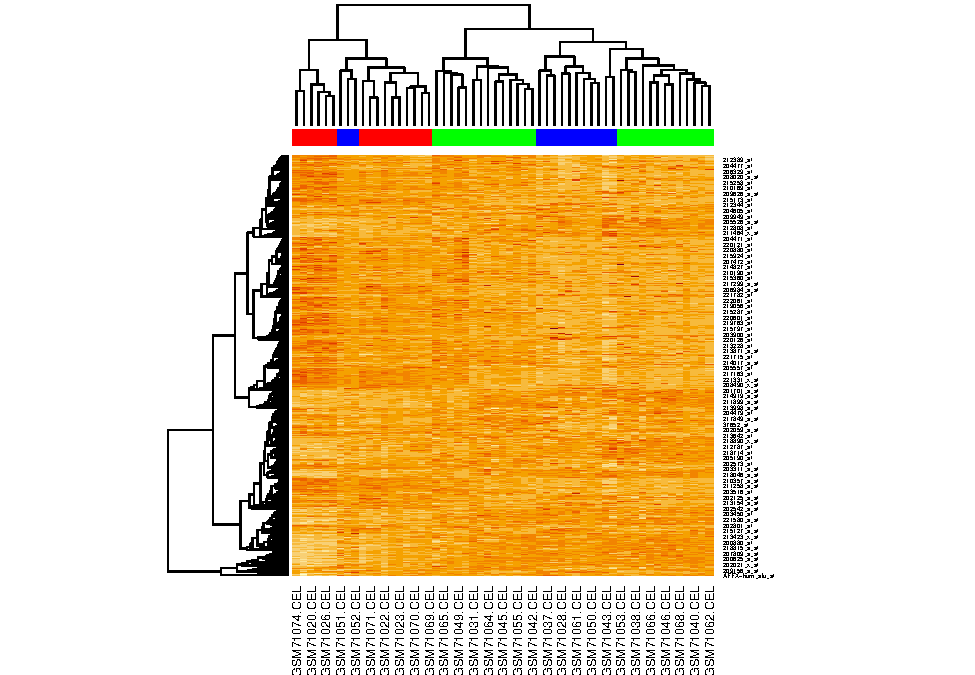
\includegraphics{_main_files/figure-latex/heatmap-bladder1-1.pdf}

Why aren't the samples clustering?

Now try providing the \texttt{hclustfun} to \texttt{heatmap()} so it uses the same method to cluster as we did. For this we will create a custom function:

\begin{Shaded}
\begin{Highlighting}[]
\NormalTok{myhclust }\OtherTok{\textless{}{-}} \ControlFlowTok{function}\NormalTok{(x) \{}
    \FunctionTok{hclust}\NormalTok{(x,}\AttributeTok{method=}\StringTok{"ward.D2"}\NormalTok{)}
\NormalTok{\}}
\end{Highlighting}
\end{Shaded}

And now we run heatmap again, using our clustering function:

\begin{Shaded}
\begin{Highlighting}[]
\FunctionTok{heatmap}\NormalTok{(bexprs,}
    \AttributeTok{ColSideColors=}\NormalTok{clust\_colours,}
    \AttributeTok{hclustfun=}\NormalTok{myhclust}
\NormalTok{)}
\end{Highlighting}
\end{Shaded}

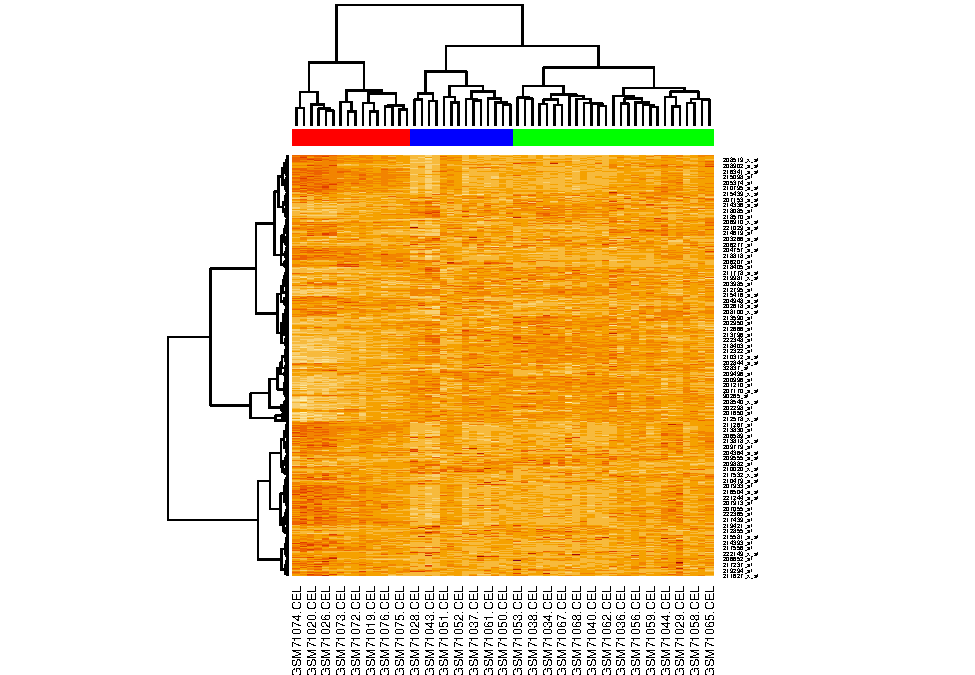
\includegraphics{_main_files/figure-latex/heatmap-bladder2-1.pdf}

\subsection{K-means Clustering}\label{k-means-clustering}

Let's try using k-means clustering, asking for three clusters:

\begin{Shaded}
\begin{Highlighting}[]
\NormalTok{kclust }\OtherTok{\textless{}{-}} \FunctionTok{kmeans}\NormalTok{(}
\NormalTok{    mouse\_exp, }
    \AttributeTok{centers =} \DecValTok{3}
\NormalTok{)}
\NormalTok{kclust}
\end{Highlighting}
\end{Shaded}

\begin{verbatim}
## K-means clustering with 3 clusters of sizes 61, 64, 22
## 
## Cluster means:
##         M1       M2       M3      NC1      NC2      NC3
## 1 3.947440 3.946048 4.012209 3.922949 3.950984 4.004362
## 2 5.553148 5.499583 5.642404 5.426931 5.435363 5.353342
## 3 7.416536 7.406216 7.414799 7.548674 7.534414 7.520608
## 
## Clustering vector:
##   1   2   3   4   5   6   7   8   9  10  11  12  13  14  15  16  17  18  19  20 
##   2   1   1   2   2   1   2   2   2   1   3   1   2   3   1   2   3   3   1   2 
##  21  22  23  24  25  26  27  28  29  30  31  32  33  34  35  36  37  38  39  40 
##   2   2   1   1   1   1   3   2   1   2   2   3   1   2   2   1   1   1   2   1 
##  41  42  43  44  45  46  47  48  49  50  51  52  53  54  55  56  57  58  59  60 
##   2   3   3   1   1   3   1   1   1   1   2   1   3   3   2   2   1   1   2   1 
##  61  62  63  64  65  66  67  68  69  70  71  72  73  74  75  76  77  78  79  80 
##   1   3   2   1   2   1   2   3   2   1   2   2   2   2   2   3   1   1   2   3 
##  81  82  83  84  85  86  87  88  89  90  91  92  93  94  95  96  97  98  99 100 
##   2   3   1   2   2   1   3   2   1   2   1   1   1   1   1   1   1   2   1   2 
## 101 102 103 104 105 106 107 108 109 110 111 112 113 114 115 116 117 118 119 120 
##   1   2   1   1   1   1   3   2   1   2   2   1   2   2   2   2   3   3   1   2 
## 121 122 123 124 125 126 127 128 129 130 131 132 133 134 135 136 137 138 139 140 
##   2   2   3   1   2   2   2   1   2   2   2   2   2   1   1   1   1   1   1   2 
## 141 142 143 144 145 146 147 
##   2   1   2   3   2   2   2 
## 
## Within cluster sum of squares by cluster:
## [1] 193.59229 166.24343  81.44264
##  (between_SS / total_SS =  74.3 %)
## 
## Available components:
## 
## [1] "cluster"      "centers"      "totss"        "withinss"     "tot.withinss"
## [6] "betweenss"    "size"         "iter"         "ifault"
\end{verbatim}

\subsection{\texorpdfstring{Using \texttt{clValid} to Determine Number of Clusters}{Using clValid to Determine Number of Clusters}}\label{using-clvalid-to-determine-number-of-clusters}

Use the \texttt{clValid()} function to validate clusters using the:

\begin{itemize}
\tightlist
\item
  Dunn index,
\item
  silhouette scores, and
\item
  connectivity
\end{itemize}

\begin{Shaded}
\begin{Highlighting}[]
\NormalTok{validation\_data }\OtherTok{\textless{}{-}} \FunctionTok{clValid}\NormalTok{(}
\NormalTok{    mouse\_exp,}
    \DecValTok{2}\SpecialCharTok{:}\DecValTok{6}\NormalTok{, }\CommentTok{\# num. clusters to evaluate}
    \AttributeTok{clMethods =} \FunctionTok{c}\NormalTok{(}\StringTok{"hier"}\NormalTok{,}\StringTok{"kmeans"}\NormalTok{), }\CommentTok{\# methods to eval.}
    \AttributeTok{validation =} \StringTok{"internal"}
\NormalTok{)}
\end{Highlighting}
\end{Shaded}

Let's look at the results:

\begin{Shaded}
\begin{Highlighting}[]
\FunctionTok{summary}\NormalTok{(validation\_data)}
\end{Highlighting}
\end{Shaded}

\begin{verbatim}
## 
## Clustering Methods:
##  hierarchical kmeans 
## 
## Cluster sizes:
##  2 3 4 5 6 
## 
## Validation Measures:
##                                  2       3       4       5       6
##                                                                   
## hierarchical Connectivity   5.3270 14.2528 20.7520 27.0726 30.6194
##              Dunn           0.1291  0.0788  0.0857  0.0899  0.0899
##              Silhouette     0.5133  0.4195  0.3700  0.3343  0.3233
## kmeans       Connectivity  13.2548 17.6651 37.3980 43.2655 50.6095
##              Dunn           0.0464  0.0873  0.0777  0.0815  0.0703
##              Silhouette     0.4571  0.4182  0.3615  0.3367  0.3207
## 
## Optimal Scores:
## 
##              Score  Method       Clusters
## Connectivity 5.3270 hierarchical 2       
## Dunn         0.1291 hierarchical 2       
## Silhouette   0.5133 hierarchical 2
\end{verbatim}

All measures of clustering consistently indicate that \textbf{two} clusters best fit the data.

Now let's cluster:

\begin{Shaded}
\begin{Highlighting}[]
\NormalTok{d }\OtherTok{\textless{}{-}} \FunctionTok{dist}\NormalTok{(}\FunctionTok{t}\NormalTok{(}\FunctionTok{log}\NormalTok{(mouse\_exp)))}
\NormalTok{h }\OtherTok{\textless{}{-}} \FunctionTok{hclust}\NormalTok{(d,}\AttributeTok{method=}\StringTok{"ward.D2"}\NormalTok{)}
\NormalTok{cluster\_ids }\OtherTok{\textless{}{-}} \FunctionTok{cutree}\NormalTok{(h, }\AttributeTok{k =} \DecValTok{2}\NormalTok{)}
\NormalTok{clust\_colors }\OtherTok{\textless{}{-}} \FunctionTok{c}\NormalTok{(}\StringTok{"dodgerblue"}\NormalTok{,}\StringTok{"orangered"}\NormalTok{)[cluster\_ids]}

\FunctionTok{heatmap}\NormalTok{(}
    \FunctionTok{as.matrix}\NormalTok{(mouse\_exp),}
    \AttributeTok{hclustfun =}\NormalTok{ myhclust,}
    \AttributeTok{ColSideColors =}\NormalTok{ clust\_colors}
\NormalTok{)}
\end{Highlighting}
\end{Shaded}

\includegraphics{_main_files/figure-latex/unnamed-chunk-26-1.pdf}

\subsection{Bonus Exercise}\label{bonus-exercise}

For your exercise, try the following:

\begin{itemize}
\tightlist
\item
  Load the MASS package using: \texttt{library(MASS)}
\item
  Import \texttt{crabs} dataset using: \texttt{data(crabs)}
\item
  Learn about this dataset using: \texttt{?crabs}
\item
  Extract the numeric columns describing the crab measurements (``FL'', ``RW'', ``CL'', ``CW'', ``BD'')
\item
  Cluster the numeric columns using your method of choice
\item
  Plot and color your data by clusters, by species (\texttt{sp}), and \texttt{sex}
\item
  Do your clusters seem to separate these groups in the same way?
\end{itemize}

\subsection{Bonus Exercise Results}\label{bonus-exercise-results}

Load packages and data, subset needed columns:

\begin{Shaded}
\begin{Highlighting}[]
\FunctionTok{library}\NormalTok{(MASS)}
\FunctionTok{data}\NormalTok{(crabs)}
\end{Highlighting}
\end{Shaded}

Learn more about the data:

\begin{Shaded}
\begin{Highlighting}[]
\NormalTok{?crabs}
\FunctionTok{head}\NormalTok{(crabs)}
\end{Highlighting}
\end{Shaded}

\begin{verbatim}
##   sp sex index   FL  RW   CL   CW  BD
## 1  B   M     1  8.1 6.7 16.1 19.0 7.0
## 2  B   M     2  8.8 7.7 18.1 20.8 7.4
## 3  B   M     3  9.2 7.8 19.0 22.4 7.7
## 4  B   M     4  9.6 7.9 20.1 23.1 8.2
## 5  B   M     5  9.8 8.0 20.3 23.0 8.2
## 6  B   M     6 10.8 9.0 23.0 26.5 9.8
\end{verbatim}

Subset needed columns:

\begin{Shaded}
\begin{Highlighting}[]
\NormalTok{crabs\_meas }\OtherTok{\textless{}{-}}\NormalTok{  crabs[,}\FunctionTok{c}\NormalTok{(}\StringTok{"FL"}\NormalTok{,}\StringTok{"RW"}\NormalTok{,}\StringTok{"CL"}\NormalTok{,}\StringTok{"CW"}\NormalTok{,}\StringTok{"BD"}\NormalTok{)]}
\end{Highlighting}
\end{Shaded}

Perform hierarchical clustering:

\begin{Shaded}
\begin{Highlighting}[]
\NormalTok{c\_dist }\OtherTok{\textless{}{-}} \FunctionTok{dist}\NormalTok{(crabs\_meas)}
\NormalTok{c\_hclust }\OtherTok{\textless{}{-}} \FunctionTok{hclust}\NormalTok{(c\_dist)}
\FunctionTok{plot}\NormalTok{(c\_hclust)}
\end{Highlighting}
\end{Shaded}

\includegraphics{_main_files/figure-latex/unnamed-chunk-30-1.pdf}

Colour-code samples based on cluster assignment. Assume there are two clusters.

\begin{Shaded}
\begin{Highlighting}[]
\NormalTok{c\_clusters }\OtherTok{=} \FunctionTok{cutree}\NormalTok{(c\_hclust,}\AttributeTok{k =} \DecValTok{2}\NormalTok{)}
\end{Highlighting}
\end{Shaded}

Now create a pairs plot, but colour-code by:

\begin{enumerate}
\def\labelenumi{\arabic{enumi}.}
\tightlist
\item
  by gene-expression based clusters
\item
  by species
\item
  by sex
\end{enumerate}

\begin{Shaded}
\begin{Highlighting}[]
\FunctionTok{pairs}\NormalTok{(}
\NormalTok{    crabs\_meas, }
    \AttributeTok{col =} \FunctionTok{c}\NormalTok{(}\StringTok{"orchid"}\NormalTok{,}\StringTok{"forestgreen"}\NormalTok{)[c\_clusters]}
\NormalTok{)}
\end{Highlighting}
\end{Shaded}

\includegraphics{_main_files/figure-latex/unnamed-chunk-32-1.pdf}

\begin{Shaded}
\begin{Highlighting}[]
\FunctionTok{pairs}\NormalTok{(}
\NormalTok{    crabs\_meas, }
    \AttributeTok{col =} \FunctionTok{c}\NormalTok{(}\StringTok{"orchid"}\NormalTok{,}\StringTok{"forestgreen"}\NormalTok{)[}\FunctionTok{factor}\NormalTok{(crabs}\SpecialCharTok{$}\NormalTok{sp)]}
\NormalTok{)}
\end{Highlighting}
\end{Shaded}

\includegraphics{_main_files/figure-latex/unnamed-chunk-32-2.pdf}

\begin{Shaded}
\begin{Highlighting}[]
\FunctionTok{pairs}\NormalTok{(}
\NormalTok{    crabs\_meas, }
    \AttributeTok{col =} \FunctionTok{c}\NormalTok{(}\StringTok{"orchid"}\NormalTok{,}\StringTok{"forestgreen"}\NormalTok{)[}\FunctionTok{factor}\NormalTok{(crabs}\SpecialCharTok{$}\NormalTok{sex)]}
\NormalTok{)}
\end{Highlighting}
\end{Shaded}

\includegraphics{_main_files/figure-latex/unnamed-chunk-32-3.pdf}

Hierarchical clustering:

\begin{Shaded}
\begin{Highlighting}[]
\NormalTok{h }\OtherTok{\textless{}{-}} \FunctionTok{hclust}\NormalTok{(}\FunctionTok{dist}\NormalTok{(crabs\_meas),}\AttributeTok{method=}\StringTok{"ward.D2"}\NormalTok{)}
\NormalTok{c2 }\OtherTok{\textless{}{-}} \FunctionTok{cutree}\NormalTok{(h,}\AttributeTok{k=}\DecValTok{2}\NormalTok{)}

\NormalTok{hclust\_fun }\OtherTok{\textless{}{-}} \ControlFlowTok{function}\NormalTok{(x)\{}
\NormalTok{    f }\OtherTok{\textless{}{-}} \FunctionTok{hclust}\NormalTok{(x, }\AttributeTok{method =} \StringTok{"ward.D2"}\NormalTok{);}
    \FunctionTok{return}\NormalTok{(f)}
\NormalTok{\}}

\FunctionTok{library}\NormalTok{(RColorBrewer)}
\FunctionTok{heatmap}\NormalTok{(}
    \FunctionTok{as.matrix}\NormalTok{(crabs\_meas),}
    \AttributeTok{hclustfun =}\NormalTok{ hclust\_fun,}
    \AttributeTok{col =} \FunctionTok{brewer.pal}\NormalTok{(}\StringTok{"Blues"}\NormalTok{,}\AttributeTok{n=}\DecValTok{8}\NormalTok{),}
    \AttributeTok{RowSideColors =} \FunctionTok{c}\NormalTok{(}\StringTok{"pink"}\NormalTok{,}\StringTok{"brown"}\NormalTok{)[c2], }
    \AttributeTok{ColSideColors =} \FunctionTok{rep}\NormalTok{(}\StringTok{"green"}\NormalTok{,}\DecValTok{5}\NormalTok{)}
\NormalTok{)}
\end{Highlighting}
\end{Shaded}

\includegraphics{_main_files/figure-latex/unnamed-chunk-33-1.pdf}

Plot by sex:

\begin{Shaded}
\begin{Highlighting}[]
\FunctionTok{heatmap}\NormalTok{(}
    \FunctionTok{as.matrix}\NormalTok{(crabs\_meas),}
    \AttributeTok{hclustfun =}\NormalTok{ hclust\_fun,}
    \AttributeTok{col =} \FunctionTok{brewer.pal}\NormalTok{(}\StringTok{"Blues"}\NormalTok{,}\AttributeTok{n=}\DecValTok{8}\NormalTok{),}
    \AttributeTok{RowSideColors =} \FunctionTok{c}\NormalTok{(}\StringTok{"pink"}\NormalTok{,}\StringTok{"brown"}\NormalTok{)[}\FunctionTok{factor}\NormalTok{(crabs}\SpecialCharTok{$}\NormalTok{sex)], }
    \AttributeTok{ColSideColors =} \FunctionTok{rep}\NormalTok{(}\StringTok{"green"}\NormalTok{,}\DecValTok{5}\NormalTok{)}
\NormalTok{)}
\end{Highlighting}
\end{Shaded}

\includegraphics{_main_files/figure-latex/unnamed-chunk-34-1.pdf}

\chapter{Module 2: Dimensionality Reduction}\label{module-2-dimensionality-reduction}

\section{Lecture}\label{lecture-1}

\includegraphics[width=1\textwidth,height=9.375in]{content-files/module-2-lecture.pdf}\\

\section{Lab}\label{lab-1}

The goal of this lab is to learn how to reduce the dimension of your dataset.

We will learn three different methods commonly used for dimension reduction:

\begin{enumerate}
\def\labelenumi{\arabic{enumi}.}
\tightlist
\item
  Principal Component Analysis
\item
  t-stochastic Neighbor Embedding (tSNE)
\item
  Uniform Manifold Approximation (UMAP)
\end{enumerate}

\subsection{Principal Component Analysis}\label{principal-component-analysis}

Let's start with PCA. PCA is commonly used as one step in a series of analyses. The goal of PCA is to explain most of the variability in the data with a smaller number of variables than the original data set. You can use PCA to explain the variability in your data using fewer variables. Typically, it is useful to identify outliers and determine if there's batch effect in your data.

Data: We will use the dataset that we used for exploratory analysis in Module 1. Load the mouse data.

\begin{Shaded}
\begin{Highlighting}[]
\FunctionTok{library}\NormalTok{(clValid)}
\FunctionTok{data}\NormalTok{(}\StringTok{"mouse"}\NormalTok{)}
\NormalTok{mouse\_exp }\OtherTok{\textless{}{-}}\NormalTok{ mouse[,}\FunctionTok{c}\NormalTok{(}\StringTok{"M1"}\NormalTok{,}\StringTok{"M2"}\NormalTok{,}\StringTok{"M3"}\NormalTok{,}\StringTok{"NC1"}\NormalTok{,}\StringTok{"NC2"}\NormalTok{,}\StringTok{"NC3"}\NormalTok{)]}
\FunctionTok{head}\NormalTok{(mouse\_exp)}
\end{Highlighting}
\end{Shaded}

\begin{verbatim}
##         M1       M2       M3      NC1      NC2      NC3
## 1 4.706812 4.528291 4.325836 5.568435 6.915079 7.353144
## 2 3.867962 4.052354 3.474651 4.995836 5.056199 5.183585
## 3 2.875112 3.379619 3.239800 3.877053 4.459629 4.850978
## 4 5.326943 5.498930 5.629814 6.795194 6.535522 6.622577
## 5 5.370125 4.546810 5.704810 6.407555 6.310487 6.195847
## 6 3.471347 4.129992 3.964431 4.474737 5.185631 5.177967
\end{verbatim}

\subsubsection{Step 1. Preparing our Data}\label{step-1.-preparing-our-data}

It is important to make sure that all the variables in your dataset are on the same scale to ensure they are comparable. So, let us check if that is the case with our dataset. To do that, we will first compute the means and variances of each variable using \texttt{apply()}.

\begin{Shaded}
\begin{Highlighting}[]
\FunctionTok{apply}\NormalTok{(mouse\_exp, }\DecValTok{2}\NormalTok{, mean)}
\end{Highlighting}
\end{Shaded}

\begin{verbatim}
##       M1       M2       M3      NC1      NC2      NC3 
## 5.165708 5.140265 5.231185 5.120369 5.133540 5.117914
\end{verbatim}

\begin{Shaded}
\begin{Highlighting}[]
\FunctionTok{apply}\NormalTok{(mouse\_exp, }\DecValTok{2}\NormalTok{, var)}
\end{Highlighting}
\end{Shaded}

\begin{verbatim}
##       M1       M2       M3      NC1      NC2      NC3 
## 1.858482 1.848090 1.869578 2.005517 2.080473 2.083073
\end{verbatim}

As you can see, the means and variances for all the six variables are almost the same and on the same scale, which is great!

However, keep in mind that, the variables need not always be on the same scale in other non-omics datasets. PCA is influenced by the magnitude of each variable. So, it is important to include a scaling step during data preparation. Ideally, it is great to have variables centered at zero for PCA because it makes comparing each principal component to the mean straightforward. Scaling can be done either using \texttt{scale()}.

\subsubsection{Step 2. Apply PCA}\label{step-2.-apply-pca}

Since our variables are on the same scale, we can directly apply PCA using \texttt{prcomp()}.

\begin{Shaded}
\begin{Highlighting}[]
\NormalTok{pc\_out }\OtherTok{\textless{}{-}} \FunctionTok{prcomp}\NormalTok{(}\FunctionTok{t}\NormalTok{(mouse\_exp))}
\end{Highlighting}
\end{Shaded}

The output of \texttt{prcomp()} is a list. Examine the internal structure of \texttt{pc\_out}.

\begin{Shaded}
\begin{Highlighting}[]
\FunctionTok{str}\NormalTok{(pc\_out)}
\end{Highlighting}
\end{Shaded}

\begin{verbatim}
## List of 5
##  $ sdev    : num [1:6] 5.577 1.764 1.583 0.758 0.667 ...
##  $ rotation: num [1:147, 1:6] 0.218 0.128 0.127 0.111 0.101 ...
##   ..- attr(*, "dimnames")=List of 2
##   .. ..$ : chr [1:147] "1" "2" "3" "4" ...
##   .. ..$ : chr [1:6] "PC1" "PC2" "PC3" "PC4" ...
##  $ center  : Named num [1:147] 5.57 4.44 3.78 6.07 5.76 ...
##   ..- attr(*, "names")= chr [1:147] "1" "2" "3" "4" ...
##  $ scale   : logi FALSE
##  $ x       : num [1:6, 1:6] -5.09 -4.46 -5.56 3.78 5.34 ...
##   ..- attr(*, "dimnames")=List of 2
##   .. ..$ : chr [1:6] "M1" "M2" "M3" "NC1" ...
##   .. ..$ : chr [1:6] "PC1" "PC2" "PC3" "PC4" ...
##  - attr(*, "class")= chr "prcomp"
\end{verbatim}

The output of \texttt{prcomp()} contains five elements \texttt{sdev}, \texttt{rotation}, \texttt{center}, \texttt{scale} and \texttt{x}. Let us examine what each looks like.

\begin{Shaded}
\begin{Highlighting}[]
\NormalTok{pc\_out}\SpecialCharTok{$}\NormalTok{sdev}
\end{Highlighting}
\end{Shaded}

\begin{verbatim}
## [1] 5.576793e+00 1.764207e+00 1.582710e+00 7.576131e-01 6.668424e-01
## [6] 6.513478e-15
\end{verbatim}

\texttt{sddev} gives standard deviation (used for computing variance explained). We will see how in sections below.

\begin{Shaded}
\begin{Highlighting}[]
\FunctionTok{head}\NormalTok{(pc\_out}\SpecialCharTok{$}\NormalTok{rotation)}
\end{Highlighting}
\end{Shaded}

\begin{verbatim}
##         PC1         PC2         PC3         PC4          PC5           PC6
## 1 0.2175336 -0.09843120  0.24646637 -0.18360970 -0.004759212 -0.1282942645
## 2 0.1277130 -0.05971284 -0.05865888 -0.04302434  0.069398716  0.0190233560
## 3 0.1274181 -0.06356995  0.12354321  0.18188678 -0.083764114  0.0646766982
## 4 0.1113816  0.07285611 -0.05940135  0.14861908  0.016695673 -0.0008885424
## 5 0.1010094  0.24317614  0.03484815 -0.06467411  0.047649021 -0.0883151388
## 6 0.1125121 -0.05572681  0.08624863  0.17407046 -0.264955100  0.0373735665
\end{verbatim}

After PCA, the observations are expressed in new axes and the loadings are provided in \texttt{pc\_out\$rotation}. Each column of \texttt{pc\_out\$rotation} contains the corresponding principal component loading vector.

We see that there are six distinct principal components, as indicated by column names of \texttt{pc\_out\$rotation}.

\begin{Shaded}
\begin{Highlighting}[]
\NormalTok{pc\_out}\SpecialCharTok{$}\NormalTok{center}
\end{Highlighting}
\end{Shaded}

\begin{verbatim}
##        1        2        3        4        5        6        7        8 
## 5.566266 4.438431 3.780365 6.068163 5.755939 4.400684 5.160500 5.683933 
##        9       10       11       12       13       14       15       16 
## 5.021818 3.586855 7.078354 4.669260 5.831477 8.181517 4.614013 5.382728 
##       17       18       19       20       21       22       23       24 
## 7.529027 7.313685 4.547701 5.290136 5.187301 6.013839 3.985299 3.642647 
##       25       26       27       28       29       30       31       32 
## 4.154045 4.674278 8.505242 4.899224 3.882938 4.964233 5.587100 8.420071 
##       33       34       35       36       37       38       39       40 
## 4.668532 5.571026 5.341486 4.246074 4.603076 3.906143 5.290324 3.205139 
##       41       42       43       44       45       46       47       48 
## 5.501723 6.599761 7.957662 4.147284 2.674647 7.029644 4.297315 3.550112 
##       49       50       51       52       53       54       55       56 
## 4.440525 4.440604 5.233737 4.589023 6.559673 7.563419 5.203153 5.563289 
##       57       58       59       60       61       62       63       64 
## 4.172330 4.363869 5.816609 4.678070 4.538479 8.210925 5.701295 4.330346 
##       65       66       67       68       69       70       71       72 
## 5.057213 3.462456 6.015641 7.096558 5.494757 2.779979 5.011157 6.460525 
##       73       74       75       76       77       78       79       80 
## 5.065625 6.057910 5.358162 7.126652 3.547180 3.157770 5.342622 7.277169 
##       81       82       83       84       85       86       87       88 
## 6.229511 8.134572 3.942388 5.476810 6.147777 2.856113 6.580211 5.616440 
##       89       90       91       92       93       94       95       96 
## 4.708294 5.244003 2.387781 3.769301 4.025543 3.968695 3.848995 4.564350 
##       97       98       99      100      101      102      103      104 
## 4.546153 4.840263 4.257428 6.249407 3.007570 5.067437 4.271637 4.436552 
##      105      106      107      108      109      110      111      112 
## 4.231309 3.973251 6.599789 4.837524 4.322573 4.867455 5.161541 3.307676 
##      113      114      115      116      117      118      119      120 
## 6.143019 5.071244 6.177220 4.827735 7.376264 7.533733 4.374265 5.183771 
##      121      122      123      124      125      126      127      128 
## 5.625725 5.976763 8.844863 4.056325 5.954586 4.811972 4.748867 4.025010 
##      129      130      131      132      133      134      135      136 
## 5.284776 5.388265 5.895763 6.181208 6.034146 3.303646 3.136626 3.336961 
##      137      138      139      140      141      142      143      144 
## 4.592918 3.190322 3.742253 5.845806 5.574498 3.444501 5.058708 6.899120 
##      145      146      147 
## 5.868390 5.154152 5.004526
\end{verbatim}

\begin{Shaded}
\begin{Highlighting}[]
\NormalTok{pc\_out}\SpecialCharTok{$}\NormalTok{scale}
\end{Highlighting}
\end{Shaded}

\begin{verbatim}
## [1] FALSE
\end{verbatim}

The \texttt{center} and \texttt{scale} elements correspond to the means and standard deviations of the variables that were used for scaling prior to implementing PCA.

\begin{Shaded}
\begin{Highlighting}[]
\CommentTok{\# See the principal components}
\FunctionTok{dim}\NormalTok{(pc\_out}\SpecialCharTok{$}\NormalTok{x)}
\end{Highlighting}
\end{Shaded}

\begin{verbatim}
## [1] 6 6
\end{verbatim}

\begin{Shaded}
\begin{Highlighting}[]
\FunctionTok{head}\NormalTok{(pc\_out}\SpecialCharTok{$}\NormalTok{x)}
\end{Highlighting}
\end{Shaded}

\begin{verbatim}
##           PC1         PC2        PC3        PC4        PC5          PC6
## M1  -5.091712  0.07170858  0.1415984 -1.2149422  0.5781693 6.039314e-15
## M2  -4.463273 -2.78279960 -1.0114746  0.5067161 -0.2847184 5.893565e-15
## M3  -5.560192  2.16495377  1.2469598  0.6895931 -0.3109790 5.855662e-15
## NC1  3.781742  1.47081980 -2.5212675  0.2858078  0.3841018 6.158759e-15
## NC2  5.338015  0.05493898  0.2748255 -0.6551843 -1.0483358 6.282292e-15
## NC3  5.995420 -0.97962153  1.8693583  0.3880095  0.6817622 5.522265e-15
\end{verbatim}

Let's now see the summary of the analysis using the \texttt{summary()} function!

\begin{Shaded}
\begin{Highlighting}[]
\FunctionTok{summary}\NormalTok{(pc\_out)}
\end{Highlighting}
\end{Shaded}

\begin{verbatim}
## Importance of components:
##                           PC1     PC2     PC3     PC4     PC5       PC6
## Standard deviation     5.5768 1.76421 1.58271 0.75761 0.66684 6.513e-15
## Proportion of Variance 0.8242 0.08248 0.06638 0.01521 0.01178 0.000e+00
## Cumulative Proportion  0.8242 0.90663 0.97301 0.98822 1.00000 1.000e+00
\end{verbatim}

The first row gives the \texttt{Standard\ deviation} of each component, which is the same as the result of \texttt{pc\_out\$sdev}.

The second row, \texttt{Proportion\ of\ Variance}, shows the percentage of explained variance, also obtained as variance/sum(variance) where variance is the square of sdev.

Compute variance

\begin{Shaded}
\begin{Highlighting}[]
\NormalTok{pc\_out}\SpecialCharTok{$}\NormalTok{sdev}\SpecialCharTok{\^{}}\DecValTok{2} \SpecialCharTok{/} \FunctionTok{sum}\NormalTok{(pc\_out}\SpecialCharTok{$}\NormalTok{sdev}\SpecialCharTok{\^{}}\DecValTok{2}\NormalTok{)}
\end{Highlighting}
\end{Shaded}

\begin{verbatim}
## [1] 8.241484e-01 8.247748e-02 6.638030e-02 1.521008e-02 1.178373e-02
## [6] 1.124249e-30
\end{verbatim}

From the second row you can see that the first principal component explains over 82.4\% of the total variance (Note: multiply each number by 100 to get the percentages).

The second principal component explains 8.2\% of the variance, and the amount of variance explained reduces further down with each component.

Finally, the last row, \texttt{Cumulative\ Proportion}, calculates the cumulative sum of the second row.

Now, let's have some fun with visualising the results of PCA.

\subsubsection{Step 3. Visualisation of PCA Results}\label{step-3.-visualisation-of-pca-results}

\textbf{A. Scree Plot}

We can visualize the percentage of explained variance per principal component by using what is called a scree plot. We will call the \texttt{fviz\_eig()} function of the factoextra package for the application. You may need to install the package using \texttt{install.packages("factoextra")}.

\begin{Shaded}
\begin{Highlighting}[]
\FunctionTok{library}\NormalTok{(factoextra)}
\FunctionTok{fviz\_eig}\NormalTok{(pc\_out, }
         \AttributeTok{addlabels =} \ConstantTok{TRUE}\NormalTok{)}
\end{Highlighting}
\end{Shaded}

\includegraphics{_main_files/figure-latex/unnamed-chunk-45-1.pdf}

The x-axis shows the PCs and the y-axis shows the percentage of variance explained that we saw above. Percentages are listed on top of the bars. It's common to see that the first few principal components explain the major amount of variance.

Scree plot can also be used to decide the number of components to keep for rest of your analysis. One of the ways is using the elbow rule. This method is about looking for the ``elbow'' shape on the curve and retaining all components before the point where the curve flattens out. Here, the elbow appears to occur at the second principal component.

Note that we will NOT remove any components for the current analysis since our goal is to understand how PCA can be used to identify batch effect in the data.

\textbf{B. Scatter Plot}

After a PCA, the observations are expressed in principal component scores (as we saw above in \texttt{pc\_out\$rotation}). So, it is important to visualize the observations along the new axes (principal components) how observations have been transformed and to understand the relations in the dataset.

This can be achieved by drawing a scatterplot. To do so, first, we need to extract and the principal component scores in \texttt{pc\_out\$rotation}, and then we will store them in a data frame called PC.

\begin{Shaded}
\begin{Highlighting}[]
\NormalTok{PC }\OtherTok{\textless{}{-}} \FunctionTok{as.data.frame}\NormalTok{(pc\_out}\SpecialCharTok{$}\NormalTok{x)}
\end{Highlighting}
\end{Shaded}

Plot the first two principal components as follows:

\begin{Shaded}
\begin{Highlighting}[]
\FunctionTok{plot}\NormalTok{(}\AttributeTok{x =}\NormalTok{ PC}\SpecialCharTok{$}\NormalTok{PC1,}
     \AttributeTok{y =}\NormalTok{ PC}\SpecialCharTok{$}\NormalTok{PC2,}
     \AttributeTok{pch =} \DecValTok{19}\NormalTok{,}
     \AttributeTok{xlab=}\StringTok{"PC1"}\NormalTok{,}
     \AttributeTok{ylab=}\StringTok{"PC2"}\NormalTok{)}
\end{Highlighting}
\end{Shaded}

\includegraphics{_main_files/figure-latex/unnamed-chunk-47-1.pdf}

We see six points in two different groups. The points correspond to six samples. But, we don't know what group/condition they belong to.

That can be done by adding sample-related information to the data.frame \texttt{PC} (such as cell type, treatment type, batch they were processed etc) as new variables. Here we will add the sample names and the cell types.

\begin{Shaded}
\begin{Highlighting}[]
\NormalTok{PC}\SpecialCharTok{$}\NormalTok{sample }\OtherTok{\textless{}{-}} \FunctionTok{factor}\NormalTok{(}\FunctionTok{rownames}\NormalTok{(PC))}
\NormalTok{PC}\SpecialCharTok{$}\NormalTok{cells }\OtherTok{\textless{}{-}} \FunctionTok{factor}\NormalTok{(}\FunctionTok{c}\NormalTok{(}\FunctionTok{rep}\NormalTok{(}\StringTok{"mesoderm"}\NormalTok{, }\DecValTok{3}\NormalTok{), }\FunctionTok{rep}\NormalTok{(}\StringTok{"neural\_crest"}\NormalTok{, }\DecValTok{3}\NormalTok{)))}
\end{Highlighting}
\end{Shaded}

Plot the scatterplot again and now, colour the points by cell type. Then, add sample names and legend.

\begin{Shaded}
\begin{Highlighting}[]
\FunctionTok{plot}\NormalTok{(}\AttributeTok{x =}\NormalTok{ PC}\SpecialCharTok{$}\NormalTok{PC1,}
     \AttributeTok{y =}\NormalTok{ PC}\SpecialCharTok{$}\NormalTok{PC2,}
     \AttributeTok{col =}\NormalTok{ PC}\SpecialCharTok{$}\NormalTok{cells,}
     \AttributeTok{pch =} \DecValTok{19}\NormalTok{,}
     \AttributeTok{xlab=}\StringTok{"PC1"}\NormalTok{,}
     \AttributeTok{ylab=}\StringTok{"PC2"}\NormalTok{)}

\FunctionTok{text}\NormalTok{(}\AttributeTok{x=}\NormalTok{ PC}\SpecialCharTok{$}\NormalTok{PC1,}
     \AttributeTok{y =}\NormalTok{ PC}\SpecialCharTok{$}\NormalTok{PC2}\FloatTok{{-}0.15}\NormalTok{,}
     \AttributeTok{labels =}\NormalTok{ PC}\SpecialCharTok{$}\NormalTok{sample)}

\FunctionTok{legend}\NormalTok{(}\StringTok{"bottomright"}\NormalTok{, }
       \AttributeTok{legend =} \FunctionTok{levels}\NormalTok{(PC}\SpecialCharTok{$}\NormalTok{cells), }
       \AttributeTok{col =} \FunctionTok{seq\_along}\NormalTok{(}\FunctionTok{levels}\NormalTok{(PC}\SpecialCharTok{$}\NormalTok{cells)), }
       \AttributeTok{pch =} \DecValTok{19}\NormalTok{)}
\end{Highlighting}
\end{Shaded}

\includegraphics{_main_files/figure-latex/unnamed-chunk-49-1.pdf}

Samples from each cell type are closer together on the scatter plot. If the batch information is available, it can also be used to colour the scatterplot. Ideally, samples from different conditions should cluster together, irrespective of the batch they were processed in.

You can also plot other PCs such as PC2 vs PC3 by changing the x and y variables above. Another way to plot all PCs is using \texttt{pairs()}

\begin{Shaded}
\begin{Highlighting}[]
\FunctionTok{pairs}\NormalTok{(PC[,}\DecValTok{1}\SpecialCharTok{:}\DecValTok{6}\NormalTok{], }
      \AttributeTok{col=}\FunctionTok{c}\NormalTok{(}\StringTok{"black"}\NormalTok{,}\StringTok{"red"}\NormalTok{)[PC}\SpecialCharTok{$}\NormalTok{cells], }
      \AttributeTok{pch=}\DecValTok{16}\NormalTok{)}
\end{Highlighting}
\end{Shaded}

\includegraphics{_main_files/figure-latex/unnamed-chunk-50-1.pdf}

\textbf{C. Biplot}

Another useful plots to understand the results are biplots. We will use the \texttt{fviz\_pca\_biplot()} function of the factoextra package. We will set label=``var'' argument to label the variables.

\begin{Shaded}
\begin{Highlighting}[]
\FunctionTok{fviz\_pca\_biplot}\NormalTok{(pc\_out, }\AttributeTok{label =} \StringTok{"var"}\NormalTok{)}
\end{Highlighting}
\end{Shaded}

\includegraphics{_main_files/figure-latex/unnamed-chunk-51-1.pdf}

The axes show the principal component scores, and the vectors are the loading vectors, whose components are in the magnitudes of the loadings. Vectors indicate that samples from each cell type are closer together.

\subsection{t-Distributed Stochastic Neighbor Embedding (t-SNE)}\label{t-distributed-stochastic-neighbor-embedding-t-sne}

t-SNE is a technique for dimensionality reduction that is particularly well suited for the visualization of high-dimensional datasets.

There are several packages that have implemented t-SNE. Here we are going to use the package \texttt{tsne} and the function \texttt{tsne}. Let's run the t-SNE algorithm on the iris dataset and generate a t-SNE plot.

\begin{Shaded}
\begin{Highlighting}[]
\FunctionTok{library}\NormalTok{(tsne)}
\FunctionTok{library}\NormalTok{(RColorBrewer)}

\DocumentationTok{\#\#\# load the input data}
\FunctionTok{data}\NormalTok{(iris)}
\NormalTok{iris\_data }\OtherTok{\textless{}{-}}\NormalTok{ iris[,}\SpecialCharTok{{-}}\DecValTok{5}\NormalTok{]}

\CommentTok{\# set colours of the plot}
\NormalTok{my\_cols\_vec }\OtherTok{\textless{}{-}} \FunctionTok{brewer.pal}\NormalTok{(}\StringTok{"Set1"}\NormalTok{,}\AttributeTok{n =} \FunctionTok{length}\NormalTok{(}\FunctionTok{levels}\NormalTok{(iris}\SpecialCharTok{$}\NormalTok{Species)))}
\NormalTok{species\_cols }\OtherTok{\textless{}{-}}\NormalTok{ my\_cols\_vec[}\FunctionTok{factor}\NormalTok{(iris}\SpecialCharTok{$}\NormalTok{Species)]}

\CommentTok{\# run t{-}SNE}
\NormalTok{iris\_tsne }\OtherTok{\textless{}{-}} \FunctionTok{tsne}\NormalTok{(iris\_data)}

\FunctionTok{plot}\NormalTok{(iris\_tsne,}
     \AttributeTok{pch=}\DecValTok{16}\NormalTok{, }
     \AttributeTok{col=}\NormalTok{species\_cols)}
\FunctionTok{legend}\NormalTok{(}\StringTok{"topright"}\NormalTok{,}
       \AttributeTok{legend =} \FunctionTok{levels}\NormalTok{(iris}\SpecialCharTok{$}\NormalTok{Species),}
       \AttributeTok{col =}\NormalTok{ my\_cols\_vec,}
       \AttributeTok{pch =} \DecValTok{19}\NormalTok{)}
\end{Highlighting}
\end{Shaded}

\includegraphics{_main_files/figure-latex/unnamed-chunk-52-1.pdf}

The \texttt{tsne} function has a parameter called \texttt{perplexity} which determines how to balance attention to neighborhood vs global structure. Default value is 30 which was used above. Set perplexity to 10, 20, 50, 100 and rerun tsne. Then visualise each result.

\begin{Shaded}
\begin{Highlighting}[]
\NormalTok{iris\_tsne10 }\OtherTok{\textless{}{-}} \FunctionTok{tsne}\NormalTok{(iris\_data,}\AttributeTok{perplexity =} \DecValTok{10}\NormalTok{)}
\NormalTok{iris\_tsne20 }\OtherTok{\textless{}{-}} \FunctionTok{tsne}\NormalTok{(iris\_data,}\AttributeTok{perplexity =} \DecValTok{20}\NormalTok{)}
\NormalTok{iris\_tsne50 }\OtherTok{\textless{}{-}} \FunctionTok{tsne}\NormalTok{(iris\_data,}\AttributeTok{perplexity =} \DecValTok{50}\NormalTok{)}
\NormalTok{iris\_tsne100 }\OtherTok{\textless{}{-}} \FunctionTok{tsne}\NormalTok{(iris\_data,}\AttributeTok{perplexity =} \DecValTok{100}\NormalTok{)}
\end{Highlighting}
\end{Shaded}

\begin{Shaded}
\begin{Highlighting}[]
\FunctionTok{par}\NormalTok{(}\AttributeTok{mfrow=}\FunctionTok{c}\NormalTok{(}\DecValTok{2}\NormalTok{,}\DecValTok{2}\NormalTok{))}

\FunctionTok{plot}\NormalTok{(iris\_tsne10[,}\DecValTok{1}\NormalTok{],}
\NormalTok{     iris\_tsne10[,}\DecValTok{2}\NormalTok{],}
     \AttributeTok{main =} \StringTok{"Perplexity = 10"}\NormalTok{,}
     \AttributeTok{col =}\NormalTok{ species\_cols,}
     \AttributeTok{pch=}\DecValTok{16}\NormalTok{)}

\FunctionTok{plot}\NormalTok{(iris\_tsne20[,}\DecValTok{1}\NormalTok{],}
\NormalTok{     iris\_tsne20[,}\DecValTok{2}\NormalTok{],}
     \AttributeTok{main =} \StringTok{"Perplexity = 20"}\NormalTok{,}
     \AttributeTok{col =}\NormalTok{ species\_cols,}
     \AttributeTok{pch=}\DecValTok{16}\NormalTok{)}

\FunctionTok{plot}\NormalTok{(iris\_tsne50[,}\DecValTok{1}\NormalTok{],}
\NormalTok{     iris\_tsne50[,}\DecValTok{2}\NormalTok{],}
     \AttributeTok{main =} \StringTok{"Perplexity = 50"}\NormalTok{,}
     \AttributeTok{col =}\NormalTok{ species\_cols,}
     \AttributeTok{pch=}\DecValTok{16}\NormalTok{)}

\FunctionTok{plot}\NormalTok{(iris\_tsne100[,}\DecValTok{1}\NormalTok{],}
\NormalTok{     iris\_tsne100[,}\DecValTok{2}\NormalTok{],}
     \AttributeTok{main =} \StringTok{"Perplexity = 100"}\NormalTok{,}
     \AttributeTok{col =}\NormalTok{ species\_cols,}
     \AttributeTok{pch=}\DecValTok{16}\NormalTok{)}
\end{Highlighting}
\end{Shaded}

\includegraphics{_main_files/figure-latex/unnamed-chunk-54-1.pdf}

Higher perplexity leads to higher spread in your data.

\subsection{Uniform Manifold Approximation and Projection (UMAP)}\label{uniform-manifold-approximation-and-projection-umap}

UMAP is another dimension reduction method and it uses similar neighborhood approach as t-SNE except uses Riemannian geometry.

Here we are going to use the package \texttt{umap} and the function \texttt{umap}. Let's apply UMAP on the iris dataset and generate a UMAP plot.

\begin{Shaded}
\begin{Highlighting}[]
\DocumentationTok{\#\# umap}
\FunctionTok{library}\NormalTok{(umap)}

\NormalTok{iris\_umap }\OtherTok{\textless{}{-}} \FunctionTok{umap}\NormalTok{(iris\_data)}
\FunctionTok{str}\NormalTok{(iris\_umap)}
\end{Highlighting}
\end{Shaded}

\begin{verbatim}
## List of 4
##  $ layout: num [1:150, 1:2] 15.8 17.3 17.5 17.6 15.6 ...
##  $ data  : num [1:150, 1:4] 5.1 4.9 4.7 4.6 5 5.4 4.6 5 4.4 4.9 ...
##   ..- attr(*, "dimnames")=List of 2
##   .. ..$ : NULL
##   .. ..$ : chr [1:4] "Sepal.Length" "Sepal.Width" "Petal.Length" "Petal.Width"
##  $ knn   :List of 2
##   ..$ indexes  : int [1:150, 1:15] 1 2 3 4 5 6 7 8 9 10 ...
##   ..$ distances: num [1:150, 1:15] 0 0 0 0 0 0 0 0 0 0 ...
##   ..- attr(*, "class")= chr "umap.knn"
##  $ config:List of 24
##   ..$ n_neighbors         : int 15
##   ..$ n_components        : int 2
##   ..$ metric              : chr "euclidean"
##   ..$ n_epochs            : int 200
##   ..$ input               : chr "data"
##   ..$ init                : chr "spectral"
##   ..$ min_dist            : num 0.1
##   ..$ set_op_mix_ratio    : num 1
##   ..$ local_connectivity  : num 1
##   ..$ bandwidth           : num 1
##   ..$ alpha               : num 1
##   ..$ gamma               : num 1
##   ..$ negative_sample_rate: int 5
##   ..$ a                   : num 1.58
##   ..$ b                   : num 0.895
##   ..$ spread              : num 1
##   ..$ random_state        : int 981281951
##   ..$ transform_state     : int NA
##   ..$ knn                 : logi NA
##   ..$ knn_repeats         : num 1
##   ..$ verbose             : logi FALSE
##   ..$ umap_learn_args     : logi NA
##   ..$ method              : chr "naive"
##   ..$ metric.function     :function (m, origin, targets)  
##   ..- attr(*, "class")= chr "umap.config"
##  - attr(*, "class")= chr "umap"
\end{verbatim}

\begin{Shaded}
\begin{Highlighting}[]
\FunctionTok{par}\NormalTok{(}\AttributeTok{mfrow=}\FunctionTok{c}\NormalTok{(}\DecValTok{1}\NormalTok{,}\DecValTok{1}\NormalTok{))}
\FunctionTok{plot}\NormalTok{(iris\_umap}\SpecialCharTok{$}\NormalTok{layout[,}\DecValTok{1}\NormalTok{],}
\NormalTok{     iris\_umap}\SpecialCharTok{$}\NormalTok{layout[,}\DecValTok{2}\NormalTok{],}
     \AttributeTok{col =}\NormalTok{ species\_cols, }\AttributeTok{pch =} \DecValTok{19}\NormalTok{)}
\end{Highlighting}
\end{Shaded}

\includegraphics{_main_files/figure-latex/unnamed-chunk-56-1.pdf}

\begin{Shaded}
\begin{Highlighting}[]
\CommentTok{\# legend("topright",}
\CommentTok{\#         legend = levels(mouse$FC),}
\CommentTok{\#         col = species\_cols,}
\CommentTok{\#         pch = 19)}
\end{Highlighting}
\end{Shaded}

\subsection{Bonus Exercise}\label{bonus-exercise-1}

For your exercise, try the following:

\begin{itemize}
\tightlist
\item
  Return to your crabs data
\item
  Compute the principle components (PCs) for the numeric columns
\item
  Plot these PCs and color them by species (``sp'') and sex
\item
  Now compute 2 t-SNE components for these data and color by species and sex
\item
  Finally compute 2 UMAP components for these data and color by species and sex
\item
  Do any of these dimensionality reduction methods seem to segregate sex/species groups?
\end{itemize}

\subsection{Bonus Exercise Results}\label{bonus-exercise-results-1}

PCA

\begin{Shaded}
\begin{Highlighting}[]
\NormalTok{c\_pcs }\OtherTok{=} \FunctionTok{prcomp}\NormalTok{(crabs\_meas)}
\end{Highlighting}
\end{Shaded}

Plot PC projections (embeddings).

\begin{Shaded}
\begin{Highlighting}[]
\FunctionTok{pairs}\NormalTok{(c\_pcs}\SpecialCharTok{$}\NormalTok{x, }\AttributeTok{col =} \FunctionTok{c}\NormalTok{(}\StringTok{"orchid"}\NormalTok{,}\StringTok{"forestgreen"}\NormalTok{)[}\FunctionTok{factor}\NormalTok{(crabs}\SpecialCharTok{$}\NormalTok{sp)])}
\end{Highlighting}
\end{Shaded}

\includegraphics{_main_files/figure-latex/unnamed-chunk-58-1.pdf}

\begin{Shaded}
\begin{Highlighting}[]
\FunctionTok{pairs}\NormalTok{(c\_pcs}\SpecialCharTok{$}\NormalTok{x, }\AttributeTok{col =} \FunctionTok{c}\NormalTok{(}\StringTok{"orchid"}\NormalTok{,}\StringTok{"forestgreen"}\NormalTok{)[}\FunctionTok{factor}\NormalTok{(crabs}\SpecialCharTok{$}\NormalTok{sex)])}
\end{Highlighting}
\end{Shaded}

\includegraphics{_main_files/figure-latex/unnamed-chunk-58-2.pdf}

tSNE:

\begin{Shaded}
\begin{Highlighting}[]
\FunctionTok{library}\NormalTok{(tsne)}
\NormalTok{c\_tsne10 }\OtherTok{=} \FunctionTok{tsne}\NormalTok{(crabs\_meas,}\AttributeTok{perplexity =} \DecValTok{10}\NormalTok{)}
\NormalTok{c\_tsne20 }\OtherTok{=} \FunctionTok{tsne}\NormalTok{(crabs\_meas,}\AttributeTok{perplexity =} \DecValTok{20}\NormalTok{)}
\NormalTok{c\_tsne50 }\OtherTok{=} \FunctionTok{tsne}\NormalTok{(crabs\_meas,}\AttributeTok{perplexity =} \DecValTok{50}\NormalTok{)}
\NormalTok{c\_tsne100 }\OtherTok{=} \FunctionTok{tsne}\NormalTok{(crabs\_meas,}\AttributeTok{perplexity =} \DecValTok{100}\NormalTok{)}
\end{Highlighting}
\end{Shaded}

sex\_cols = c(``orchid'',``forestgreen''){[}factor(crabs\$sex){]}

Color-code tSNE plot by species, try various perplexity levels:

\begin{Shaded}
\begin{Highlighting}[]
\NormalTok{species\_cols }\OtherTok{=} \FunctionTok{c}\NormalTok{(}\StringTok{"orchid"}\NormalTok{,}\StringTok{"forestgreen"}\NormalTok{)[}\FunctionTok{factor}\NormalTok{(crabs}\SpecialCharTok{$}\NormalTok{sp)]}
\FunctionTok{par}\NormalTok{(}\AttributeTok{mfrow=}\FunctionTok{c}\NormalTok{(}\DecValTok{2}\NormalTok{,}\DecValTok{2}\NormalTok{))}
\FunctionTok{plot}\NormalTok{(c\_tsne10[,}\DecValTok{1}\NormalTok{],}
\NormalTok{     c\_tsne10[,}\DecValTok{2}\NormalTok{],}
     \AttributeTok{main =} \StringTok{"Perplexity = 10"}\NormalTok{,}
     \AttributeTok{col =}\NormalTok{ species\_cols)}

\FunctionTok{plot}\NormalTok{(c\_tsne20[,}\DecValTok{1}\NormalTok{],}
\NormalTok{     c\_tsne20[,}\DecValTok{2}\NormalTok{],}
     \AttributeTok{main =} \StringTok{"Perplexity = 20"}\NormalTok{,}
     \AttributeTok{col =}\NormalTok{ species\_cols)}
\FunctionTok{plot}\NormalTok{(c\_tsne50[,}\DecValTok{1}\NormalTok{],}
\NormalTok{     c\_tsne50[,}\DecValTok{2}\NormalTok{],}
     \AttributeTok{main =} \StringTok{"Perplexity = 50"}\NormalTok{,}
     \AttributeTok{col =}\NormalTok{ species\_cols)}
\FunctionTok{plot}\NormalTok{(c\_tsne100[,}\DecValTok{1}\NormalTok{],}
\NormalTok{     c\_tsne100[,}\DecValTok{2}\NormalTok{],}
     \AttributeTok{main =} \StringTok{"Perplexity = 100"}\NormalTok{,}
     \AttributeTok{col =}\NormalTok{ species\_cols)}
\end{Highlighting}
\end{Shaded}

\includegraphics{_main_files/figure-latex/unnamed-chunk-60-1.pdf}

Now do the same, but colour-code for sex:

\begin{Shaded}
\begin{Highlighting}[]
\NormalTok{sex\_cols }\OtherTok{=} \FunctionTok{c}\NormalTok{(}\StringTok{"orchid"}\NormalTok{,}\StringTok{"forestgreen"}\NormalTok{)[}\FunctionTok{factor}\NormalTok{(crabs}\SpecialCharTok{$}\NormalTok{sex)]}
\FunctionTok{par}\NormalTok{(}\AttributeTok{mfrow=}\FunctionTok{c}\NormalTok{(}\DecValTok{2}\NormalTok{,}\DecValTok{2}\NormalTok{))}
\FunctionTok{plot}\NormalTok{(c\_tsne10[,}\DecValTok{1}\NormalTok{],}
\NormalTok{     c\_tsne10[,}\DecValTok{2}\NormalTok{],}
     \AttributeTok{main =} \StringTok{"Perplexity = 10"}\NormalTok{,}
     \AttributeTok{col =}\NormalTok{ sex\_cols)}
\FunctionTok{plot}\NormalTok{(c\_tsne20[,}\DecValTok{1}\NormalTok{],}
\NormalTok{     c\_tsne20[,}\DecValTok{2}\NormalTok{],}
     \AttributeTok{main =} \StringTok{"Perplexity = 20"}\NormalTok{,}
     \AttributeTok{col =}\NormalTok{ sex\_cols)}
\FunctionTok{plot}\NormalTok{(c\_tsne50[,}\DecValTok{1}\NormalTok{],}
\NormalTok{     c\_tsne50[,}\DecValTok{2}\NormalTok{],}
     \AttributeTok{main =} \StringTok{"Perplexity = 50"}\NormalTok{,}
     \AttributeTok{col =}\NormalTok{ sex\_cols)}
\FunctionTok{plot}\NormalTok{(c\_tsne100[,}\DecValTok{1}\NormalTok{],}
\NormalTok{     c\_tsne100[,}\DecValTok{2}\NormalTok{],}
     \AttributeTok{main =} \StringTok{"Perplexity = 100"}\NormalTok{,}
     \AttributeTok{col =}\NormalTok{ sex\_cols)}
\end{Highlighting}
\end{Shaded}

\includegraphics{_main_files/figure-latex/unnamed-chunk-61-1.pdf}

Run UMAP

\begin{Shaded}
\begin{Highlighting}[]
\FunctionTok{library}\NormalTok{(umap)}
\NormalTok{c\_umap }\OtherTok{\textless{}{-}} \FunctionTok{umap}\NormalTok{(crabs\_meas)}
\FunctionTok{str}\NormalTok{(c\_umap)}
\end{Highlighting}
\end{Shaded}

\begin{verbatim}
## List of 4
##  $ layout: num [1:200, 1:2] 2.8 2.88 2.98 3.14 3.4 ...
##   ..- attr(*, "dimnames")=List of 2
##   .. ..$ : chr [1:200] "1" "2" "3" "4" ...
##   .. ..$ : NULL
##  $ data  : num [1:200, 1:5] 8.1 8.8 9.2 9.6 9.8 10.8 11.1 11.6 11.8 11.8 ...
##   ..- attr(*, "dimnames")=List of 2
##   .. ..$ : chr [1:200] "1" "2" "3" "4" ...
##   .. ..$ : chr [1:5] "FL" "RW" "CL" "CW" ...
##  $ knn   :List of 2
##   ..$ indexes  : int [1:200, 1:15] 1 2 3 4 5 6 7 8 9 10 ...
##   .. ..- attr(*, "dimnames")=List of 2
##   .. .. ..$ : chr [1:200] "1" "2" "3" "4" ...
##   .. .. ..$ : NULL
##   ..$ distances: num [1:200, 1:15] 0 0 0 0 0 0 0 0 0 0 ...
##   .. ..- attr(*, "dimnames")=List of 2
##   .. .. ..$ : chr [1:200] "1" "2" "3" "4" ...
##   .. .. ..$ : NULL
##   ..- attr(*, "class")= chr "umap.knn"
##  $ config:List of 24
##   ..$ n_neighbors         : int 15
##   ..$ n_components        : int 2
##   ..$ metric              : chr "euclidean"
##   ..$ n_epochs            : int 200
##   ..$ input               : chr "data"
##   ..$ init                : chr "spectral"
##   ..$ min_dist            : num 0.1
##   ..$ set_op_mix_ratio    : num 1
##   ..$ local_connectivity  : num 1
##   ..$ bandwidth           : num 1
##   ..$ alpha               : num 1
##   ..$ gamma               : num 1
##   ..$ negative_sample_rate: int 5
##   ..$ a                   : num 1.58
##   ..$ b                   : num 0.895
##   ..$ spread              : num 1
##   ..$ random_state        : int 686219013
##   ..$ transform_state     : int NA
##   ..$ knn                 : logi NA
##   ..$ knn_repeats         : num 1
##   ..$ verbose             : logi FALSE
##   ..$ umap_learn_args     : logi NA
##   ..$ method              : chr "naive"
##   ..$ metric.function     :function (m, origin, targets)  
##   ..- attr(*, "class")= chr "umap.config"
##  - attr(*, "class")= chr "umap"
\end{verbatim}

\begin{Shaded}
\begin{Highlighting}[]
\FunctionTok{par}\NormalTok{(}\AttributeTok{mfrow=}\FunctionTok{c}\NormalTok{(}\DecValTok{1}\NormalTok{,}\DecValTok{2}\NormalTok{))}
\FunctionTok{plot}\NormalTok{(c\_umap}\SpecialCharTok{$}\NormalTok{layout[,}\DecValTok{1}\NormalTok{],}
\NormalTok{     c\_umap}\SpecialCharTok{$}\NormalTok{layout[,}\DecValTok{2}\NormalTok{],}
     \AttributeTok{col =}\NormalTok{ species\_cols, }\AttributeTok{pch =} \DecValTok{19}\NormalTok{, }
     \AttributeTok{main =} \StringTok{"Colored by species"}\NormalTok{)}

\FunctionTok{plot}\NormalTok{(c\_umap}\SpecialCharTok{$}\NormalTok{layout[,}\DecValTok{1}\NormalTok{],}
\NormalTok{     c\_umap}\SpecialCharTok{$}\NormalTok{layout[,}\DecValTok{2}\NormalTok{],}
     \AttributeTok{col =}\NormalTok{ sex\_cols, }\AttributeTok{pch =} \DecValTok{19}\NormalTok{, }
     \AttributeTok{main =} \StringTok{"Colored by sex"}\NormalTok{)}
\end{Highlighting}
\end{Shaded}

\includegraphics{_main_files/figure-latex/unnamed-chunk-62-1.pdf}

\chapter{Module 3: Generalized Linear Models}\label{module-3-generalized-linear-models}

\section{Lecture}\label{lecture-2}

\includegraphics[width=1\textwidth,height=9.375in]{content-files/module-3-lecture.pdf}\\

\section{Lab}\label{lab-2}

In this module we're going to cover:

\begin{itemize}
\tightlist
\item
  Reading data from files and evaluating missingness
\item
  Creating publication-quality plots with \texttt{ggplot2}
\item
  Fitting models with binary outcomes using generalized linear models
\end{itemize}

\subsection{Essential R: Reading Tables From Files, Merging, Basic Data Exploration}\label{essential-r-reading-tables-from-files-merging-basic-data-exploration}

For this we're going to use two data files available in the course data directory.

Download the following datasets and put them in your R working directory.

\begin{itemize}
\tightlist
\item
  \texttt{tomerge1.csv} : comma-separated values
\item
  \texttt{tomerge2.txt} : space-delimited values
\end{itemize}

Use \texttt{read.delim()} to read in tables. Note the use of the \texttt{sep=} parameter to indicate what the column separator is:

\begin{Shaded}
\begin{Highlighting}[]
\NormalTok{x1 }\OtherTok{\textless{}{-}} \FunctionTok{read.delim}\NormalTok{(}\StringTok{"datasets/tomerge1.csv"}\NormalTok{,}\AttributeTok{sep=}\StringTok{","}\NormalTok{)}
\FunctionTok{head}\NormalTok{(x1)}
\end{Highlighting}
\end{Shaded}

\begin{verbatim}
##   Sample_ID Exposure Biomarker_value
## 1         A        0              35
## 2         B        0              22
## 3         C        0              91
## 4         D        0               3
## 5         E        1              56
## 6         F        1              37
\end{verbatim}

\begin{Shaded}
\begin{Highlighting}[]
\NormalTok{x2 }\OtherTok{\textless{}{-}} \FunctionTok{read.delim}\NormalTok{(}\StringTok{"datasets/tomerge2.txt"}\NormalTok{,}\AttributeTok{sep=}\StringTok{" "}\NormalTok{)}
\FunctionTok{head}\NormalTok{(x2)}
\end{Highlighting}
\end{Shaded}

\begin{verbatim}
##   sampleID Exposure_level Biomarker2_detected
## 1        A     0.65405517                   1
## 2        B     0.67202852                   0
## 3        C     0.88646372                   1
## 4        D     0.28433256                   0
## 5        E     0.04166839                   0
## 6        F     0.45263534                   1
\end{verbatim}

Use \texttt{merge()} to combine the two tables by sample ID. Note the use of \texttt{by.x} and \texttt{by.y} to tell \texttt{merge()} which columns are equivalent:

\begin{Shaded}
\begin{Highlighting}[]
\NormalTok{x\_merge }\OtherTok{\textless{}{-}} \FunctionTok{merge}\NormalTok{(x1, x2, }\AttributeTok{by.x =} \StringTok{"Sample\_ID"}\NormalTok{, }\AttributeTok{by.y =} \StringTok{"sampleID"}\NormalTok{)}
\FunctionTok{head}\NormalTok{(x\_merge)}
\end{Highlighting}
\end{Shaded}

\begin{verbatim}
##   Sample_ID Exposure Biomarker_value Exposure_level Biomarker2_detected
## 1         A        0              35     0.65405517                   1
## 2         B        0              22     0.67202852                   0
## 3         C        0              91     0.88646372                   1
## 4         D        0               3     0.28433256                   0
## 5         E        1              56     0.04166839                   0
## 6         F        1              37     0.45263534                   1
\end{verbatim}

We're going to use a popular dataset for data analysis, pertaining to survival of passengers aboard the Titanic.

Download the following dataset and put them in your R working directory.

\begin{itemize}
\tightlist
\item
  \texttt{titanic.csv}
\end{itemize}

Let's read in the data from a file:

\begin{Shaded}
\begin{Highlighting}[]
\NormalTok{dat }\OtherTok{\textless{}{-}} \FunctionTok{read.delim}\NormalTok{(}
    \StringTok{"datasets/titanic.csv"}\NormalTok{,}
    \AttributeTok{sep=}\StringTok{","} \CommentTok{\# indicate the column separator}
\NormalTok{    ) }
\end{Highlighting}
\end{Shaded}

Examine the columns:

\begin{Shaded}
\begin{Highlighting}[]
\FunctionTok{head}\NormalTok{(dat)}
\end{Highlighting}
\end{Shaded}

\begin{verbatim}
##   PassengerId Survived Pclass
## 1           1        0      3
## 2           2        1      1
## 3           3        1      3
## 4           4        1      1
## 5           5        0      3
## 6           6        0      3
##                                                  Name    Sex Age SibSp Parch
## 1                             Braund, Mr. Owen Harris   male  22     1     0
## 2 Cumings, Mrs. John Bradley (Florence Briggs Thayer) female  38     1     0
## 3                              Heikkinen, Miss. Laina female  26     0     0
## 4        Futrelle, Mrs. Jacques Heath (Lily May Peel) female  35     1     0
## 5                            Allen, Mr. William Henry   male  35     0     0
## 6                                    Moran, Mr. James   male  NA     0     0
##             Ticket    Fare Cabin Embarked
## 1        A/5 21171  7.2500              S
## 2         PC 17599 71.2833   C85        C
## 3 STON/O2. 3101282  7.9250              S
## 4           113803 53.1000  C123        S
## 5           373450  8.0500              S
## 6           330877  8.4583              Q
\end{verbatim}

Some of the columns are categorical, use \texttt{table()} to look at the tallies. Examine the columns:

\begin{Shaded}
\begin{Highlighting}[]
\FunctionTok{table}\NormalTok{(dat}\SpecialCharTok{$}\NormalTok{Survived)}
\end{Highlighting}
\end{Shaded}

\begin{verbatim}
## 
##   0   1 
## 549 342
\end{verbatim}

\begin{Shaded}
\begin{Highlighting}[]
\FunctionTok{table}\NormalTok{(dat}\SpecialCharTok{$}\NormalTok{Pclass)}
\end{Highlighting}
\end{Shaded}

\begin{verbatim}
## 
##   1   2   3 
## 216 184 491
\end{verbatim}

Use \texttt{summary()} to look at continuous-valued data:

\begin{Shaded}
\begin{Highlighting}[]
\FunctionTok{summary}\NormalTok{(dat}\SpecialCharTok{$}\NormalTok{Age)}
\end{Highlighting}
\end{Shaded}

\begin{verbatim}
##    Min. 1st Qu.  Median    Mean 3rd Qu.    Max.    NA's 
##    0.42   20.12   28.00   29.70   38.00   80.00     177
\end{verbatim}

Notice that there are 177 \texttt{NA} (missing) values for age. Let's visualize the missing data more systematically.

\subsection{Explore Missing Data}\label{explore-missing-data}

For this let's use a little script that converts a table into black and white squares to visualize missing data. For this, install the \texttt{plotrix} package.

\begin{Shaded}
\begin{Highlighting}[]
\ControlFlowTok{if}\NormalTok{ (}\SpecialCharTok{!}\FunctionTok{requireNamespace}\NormalTok{(}\StringTok{"plotrix"}\NormalTok{, }\AttributeTok{quietly =} \ConstantTok{TRUE}\NormalTok{)) }\FunctionTok{install.packages}\NormalTok{(}\StringTok{"plotrix"}\NormalTok{)}

\FunctionTok{suppressMessages}\NormalTok{(}\FunctionTok{library}\NormalTok{(plotrix))}

\CommentTok{\#\textquotesingle{} show data missingness as a chequered matrix}
\CommentTok{\#\textquotesingle{} }
\CommentTok{\#\textquotesingle{} @param x (matrix) data matrix.}
\CommentTok{\#\textquotesingle{} @param outFile (char) path to file for printing graph}
\CommentTok{\#\textquotesingle{} @param wd (numeric) width in inches}
\CommentTok{\#\textquotesingle{} @param ht (numeric) height in inches}
\CommentTok{\#\textquotesingle{} @return plots missingness matrix to file}
\CommentTok{\#\textquotesingle{} @import plotrix}
\CommentTok{\#\textquotesingle{} @export}
\NormalTok{plotMissMat }\OtherTok{\textless{}{-}} \ControlFlowTok{function}\NormalTok{(x,}\AttributeTok{xlab=}\StringTok{"columns"}\NormalTok{,}
        \AttributeTok{ylab=}\StringTok{"rows"}\NormalTok{,}\AttributeTok{border=}\ConstantTok{NA}\NormalTok{) \{}
    
\NormalTok{    x }\OtherTok{\textless{}{-}} \SpecialCharTok{!}\FunctionTok{is.na}\NormalTok{(x)}
    \FunctionTok{class}\NormalTok{(x) }\OtherTok{\textless{}{-}} \StringTok{"numeric"}
    \FunctionTok{color2D.matplot}\NormalTok{(x,}\AttributeTok{show.values=}\ConstantTok{FALSE}\NormalTok{,}\AttributeTok{axes=}\ConstantTok{FALSE}\NormalTok{,}
        \AttributeTok{cs1=}\FunctionTok{c}\NormalTok{(}\DecValTok{1}\NormalTok{,}\DecValTok{0}\NormalTok{),}\AttributeTok{cs2=}\FunctionTok{c}\NormalTok{(}\DecValTok{1}\NormalTok{,}\DecValTok{0}\NormalTok{),}\AttributeTok{cs3=}\FunctionTok{c}\NormalTok{(}\DecValTok{1}\NormalTok{,}\DecValTok{0}\NormalTok{),}\AttributeTok{border=}\NormalTok{border,}
        \AttributeTok{cex=}\FloatTok{0.8}\NormalTok{,}
        \AttributeTok{xlab=}\NormalTok{xlab,}\AttributeTok{ylab=}\NormalTok{ylab)}
\NormalTok{\}}
\end{Highlighting}
\end{Shaded}

Let's look at the missingness in the Titanic dataset. Missing data is shown as a white cell, and non-missing data is shown in black.

\begin{Shaded}
\begin{Highlighting}[]
\FunctionTok{plotMissMat}\NormalTok{(dat)}
\end{Highlighting}
\end{Shaded}

\includegraphics{_main_files/figure-latex/unnamed-chunk-71-1.pdf}

We can see a column with many missing values. This is probably the ``age'' data.
Let's count the number of missing values on a per-column level.

For this we combine \texttt{is.na()}, which returns a TRUE/FALSE value for NA values, and \texttt{colSums()} which adds up the TRUE values down the columns.

\begin{Shaded}
\begin{Highlighting}[]
\FunctionTok{colSums}\NormalTok{(}\FunctionTok{is.na}\NormalTok{(dat))}
\end{Highlighting}
\end{Shaded}

\begin{verbatim}
## PassengerId    Survived      Pclass        Name         Sex         Age 
##           0           0           0           0           0         177 
##       SibSp       Parch      Ticket        Fare       Cabin    Embarked 
##           0           0           0           0           0           0
\end{verbatim}

This confirms that \texttt{Age} is the only column with missing data.

Now let's explore the data using plots.

\subsection{\texorpdfstring{Essential R: Plots with \texttt{ggplot2}}{Essential R: Plots with ggplot2}}\label{essential-r-plots-with-ggplot2}

\texttt{ggplot2} is a popular plotting package that uses an additive paradigm to build plots.

Useful websites:
* \href{https://rstudio.github.io/cheatsheets/html/data-visualization.html}{ggplot2 cheatsheet}
* The \href{https://ggplot2.tidyverse.org/}{ggplot2 website} is a wealth of reference information, so here we just touch on the basics to get you started.

Anytime you need to generate a specific kind of plot, the website will most likely have documentation for how to achieve it.

Let's start by creating a scatterplot with two \textbf{continuous variables}. For this let's load a dataset measuring statistics around quality of life in US states in the late 70's:

\begin{Shaded}
\begin{Highlighting}[]
\NormalTok{state.x77 }\OtherTok{\textless{}{-}} \FunctionTok{as.data.frame}\NormalTok{(state.x77)}
\FunctionTok{head}\NormalTok{(state.x77)}
\end{Highlighting}
\end{Shaded}

\begin{verbatim}
##            Population Income Illiteracy Life Exp Murder HS Grad Frost   Area
## Alabama          3615   3624        2.1    69.05   15.1    41.3    20  50708
## Alaska            365   6315        1.5    69.31   11.3    66.7   152 566432
## Arizona          2212   4530        1.8    70.55    7.8    58.1    15 113417
## Arkansas         2110   3378        1.9    70.66   10.1    39.9    65  51945
## California      21198   5114        1.1    71.71   10.3    62.6    20 156361
## Colorado         2541   4884        0.7    72.06    6.8    63.9   166 103766
\end{verbatim}

Create a base plot using the \texttt{ggplot} function. Then ``add'' a scatterplot to it. Notice that the plot has been assigned to a variable named \texttt{p}.

This setup is standard for \texttt{ggplot2} and allows multiple visualizations to be applied to the same base plot.

We use \texttt{aes} to tell ggplot what the \texttt{x} and \texttt{y} axes are, and later, if we want to colour-code by a particular column.

\begin{Shaded}
\begin{Highlighting}[]
\FunctionTok{library}\NormalTok{(ggplot2)}
\NormalTok{p }\OtherTok{\textless{}{-}} \FunctionTok{ggplot}\NormalTok{(state.x77, }
    \FunctionTok{aes}\NormalTok{(}\AttributeTok{x =}\NormalTok{ Illiteracy,}\AttributeTok{y =}\NormalTok{ Income)}
\NormalTok{    )}

\NormalTok{p }\OtherTok{\textless{}{-}}\NormalTok{ p }\SpecialCharTok{+} \FunctionTok{geom\_point}\NormalTok{() }\CommentTok{\# scatter plot}
\NormalTok{p}
\end{Highlighting}
\end{Shaded}

\includegraphics{_main_files/figure-latex/load-states-data-1.pdf}

Now let's add confidence intervals:

\begin{Shaded}
\begin{Highlighting}[]
\NormalTok{p }\SpecialCharTok{+} \FunctionTok{geom\_smooth}\NormalTok{()}
\end{Highlighting}
\end{Shaded}

\begin{verbatim}
## `geom_smooth()` using method = 'loess' and formula = 'y ~ x'
\end{verbatim}

\includegraphics{_main_files/figure-latex/states-geomsmooth-1.pdf}

It looks like there is a negative relationship between illiteracy and income. We can confirm this by looking at correlation:

\begin{Shaded}
\begin{Highlighting}[]
\NormalTok{x }\OtherTok{\textless{}{-}}\NormalTok{ state.x77}\SpecialCharTok{$}\NormalTok{Illiteracy}
\NormalTok{y }\OtherTok{\textless{}{-}}\NormalTok{ state.x77}\SpecialCharTok{$}\NormalTok{Income}
\FunctionTok{cor.test}\NormalTok{(x,y)}
\end{Highlighting}
\end{Shaded}

\begin{verbatim}
## 
##  Pearson's product-moment correlation
## 
## data:  x and y
## t = -3.3668, df = 48, p-value = 0.001505
## alternative hypothesis: true correlation is not equal to 0
## 95 percent confidence interval:
##  -0.6378257 -0.1807128
## sample estimates:
##        cor 
## -0.4370752
\end{verbatim}

\begin{Shaded}
\begin{Highlighting}[]
\FunctionTok{cor.test}\NormalTok{(x,y)}\SpecialCharTok{$}\NormalTok{p.value}
\end{Highlighting}
\end{Shaded}

\begin{verbatim}
## [1] 0.001505073
\end{verbatim}

Let's now examine \textbf{categorical variables}. In the titanic set, let's look at the fare paid based on passenger class:

\begin{Shaded}
\begin{Highlighting}[]
\NormalTok{p }\OtherTok{\textless{}{-}} \FunctionTok{ggplot}\NormalTok{(dat)}
\NormalTok{p }\SpecialCharTok{+} \FunctionTok{geom\_boxplot}\NormalTok{(}
    \FunctionTok{aes}\NormalTok{(}\AttributeTok{x =} \FunctionTok{factor}\NormalTok{(Pclass), }\CommentTok{\# "factor()" makes a data column a categorical variable}
        \AttributeTok{y =}\NormalTok{ Fare))}
\end{Highlighting}
\end{Shaded}

\includegraphics{_main_files/figure-latex/boxplot-1.pdf}

We can use barplots to examine counts and proportions. Let's look at number of survivors, split by passenger class.

Here the \texttt{fill} command is used to to split each barplot by the category, ``Survived''.
So you can see number of passengers by ``Pclass'' split by survival.

\begin{Shaded}
\begin{Highlighting}[]
\NormalTok{p }\SpecialCharTok{+} \FunctionTok{geom\_bar}\NormalTok{(}
    \FunctionTok{aes}\NormalTok{(}\AttributeTok{fill=}\FunctionTok{factor}\NormalTok{(Survived), }
        \AttributeTok{x =}\NormalTok{ Pclass)}
\NormalTok{)}
\end{Highlighting}
\end{Shaded}

\includegraphics{_main_files/figure-latex/barplot-1.pdf}

The plot above shows count data. Let's convert this to proportions. We can see that the fraction of non-survivors in ``Class 3'' is high.

\begin{Shaded}
\begin{Highlighting}[]
\NormalTok{p }\SpecialCharTok{+} \FunctionTok{geom\_bar}\NormalTok{(}
    \FunctionTok{aes}\NormalTok{(}\AttributeTok{fill=}\FunctionTok{factor}\NormalTok{(Survived), }\AttributeTok{x =}\NormalTok{ Pclass),}
    \AttributeTok{position =} \StringTok{"fill"}
\NormalTok{)}
\end{Highlighting}
\end{Shaded}

\includegraphics{_main_files/figure-latex/barplot2 -1.pdf}

How about males versus females?

\begin{Shaded}
\begin{Highlighting}[]
\NormalTok{p }\SpecialCharTok{+} \FunctionTok{geom\_bar}\NormalTok{(}
    \FunctionTok{aes}\NormalTok{(}\AttributeTok{fill=}\FunctionTok{factor}\NormalTok{(Survived), }\AttributeTok{x =}\NormalTok{ Sex),}
    \AttributeTok{position =} \StringTok{"fill"}
\NormalTok{)}
\end{Highlighting}
\end{Shaded}

\includegraphics{_main_files/figure-latex/finish-titanic-1.pdf}

\textbf{Exercise for later:} Try other \texttt{ggplot} functions on these data or on a small data table of your project.
(avoid using large genomics datasets, because those are going to be harder to interpret)

\subsection{\texorpdfstring{Fit Binary Response Variable Using \texttt{glm()} and Logistic Regression}{Fit Binary Response Variable Using glm() and Logistic Regression}}\label{fit-binary-response-variable-using-glm-and-logistic-regression}

Let's fit a model to a binary outcome. For this we load a dataset that measures physiological variables in a cohort of Pima Indians.

\begin{Shaded}
\begin{Highlighting}[]
\FunctionTok{library}\NormalTok{(mlbench)}
\FunctionTok{data}\NormalTok{(PimaIndiansDiabetes2)}
\CommentTok{\# type ?PimaIndiansDiabetes2 to learn more about the dataset.}

\NormalTok{dat }\OtherTok{\textless{}{-}}\NormalTok{ PimaIndiansDiabetes2}
\FunctionTok{head}\NormalTok{(dat)}
\end{Highlighting}
\end{Shaded}

\begin{verbatim}
##   pregnant glucose pressure triceps insulin mass pedigree age diabetes
## 1        6     148       72      35      NA 33.6    0.627  50      pos
## 2        1      85       66      29      NA 26.6    0.351  31      neg
## 3        8     183       64      NA      NA 23.3    0.672  32      pos
## 4        1      89       66      23      94 28.1    0.167  21      neg
## 5        0     137       40      35     168 43.1    2.288  33      pos
## 6        5     116       74      NA      NA 25.6    0.201  30      neg
\end{verbatim}

Let's look at the impact of blood glucose levels on diabetes diagnosis.

First let's make a scatterplot. Could there be a relationship?

\begin{Shaded}
\begin{Highlighting}[]
\NormalTok{p }\OtherTok{\textless{}{-}} \FunctionTok{ggplot}\NormalTok{(dat, }\FunctionTok{aes}\NormalTok{(}\AttributeTok{x =}\NormalTok{ glucose, }\AttributeTok{y =} \FunctionTok{factor}\NormalTok{(diabetes)))}
\NormalTok{p }\SpecialCharTok{+} \FunctionTok{geom\_point}\NormalTok{()}
\end{Highlighting}
\end{Shaded}

\begin{verbatim}
## Warning: Removed 5 rows containing missing values or values outside the scale range
## (`geom_point()`).
\end{verbatim}

\includegraphics{_main_files/figure-latex/plot-diabetes-vs-glucose-1.pdf}

Could this be fit with a linear model?

Is there a continuous line that could reasonably fit the data?

\begin{Shaded}
\begin{Highlighting}[]
\NormalTok{p }\OtherTok{\textless{}{-}} \FunctionTok{ggplot}\NormalTok{(dat, }\FunctionTok{aes}\NormalTok{(}\AttributeTok{x =}\NormalTok{ glucose, }\AttributeTok{y =} \FunctionTok{factor}\NormalTok{(diabetes)))}
\NormalTok{p }\SpecialCharTok{+} \FunctionTok{geom\_point}\NormalTok{() }\SpecialCharTok{+} \FunctionTok{geom\_smooth}\NormalTok{()}
\end{Highlighting}
\end{Shaded}

\begin{verbatim}
## Warning: Removed 5 rows containing non-finite outside the scale range
## (`stat_smooth()`).
\end{verbatim}

\begin{verbatim}
## Warning: Removed 5 rows containing missing values or values outside the scale range
## (`geom_point()`).
\end{verbatim}

\includegraphics{_main_files/figure-latex/unnamed-chunk-73-1.pdf}

This is a situation where a logistic regression model would be an appropriate choice because of the binary outcome.

We're going to use \texttt{glm()} to fit a model to these data:

\begin{Shaded}
\begin{Highlighting}[]
\NormalTok{mod }\OtherTok{\textless{}{-}} \FunctionTok{glm}\NormalTok{(}\FunctionTok{factor}\NormalTok{(diabetes)}\SpecialCharTok{\textasciitilde{}}\NormalTok{glucose, }
\NormalTok{    dat,}
    \AttributeTok{family =} \StringTok{"binomial"} \CommentTok{\# set to model binary outcome}
\NormalTok{)}
\FunctionTok{summary}\NormalTok{(mod)}
\end{Highlighting}
\end{Shaded}

\begin{verbatim}
## 
## Call:
## glm(formula = factor(diabetes) ~ glucose, family = "binomial", 
##     data = dat)
## 
## Coefficients:
##              Estimate Std. Error z value Pr(>|z|)    
## (Intercept) -5.715088   0.438100  -13.04   <2e-16 ***
## glucose      0.040634   0.003382   12.01   <2e-16 ***
## ---
## Signif. codes:  0 '***' 0.001 '**' 0.01 '*' 0.05 '.' 0.1 ' ' 1
## 
## (Dispersion parameter for binomial family taken to be 1)
## 
##     Null deviance: 986.70  on 762  degrees of freedom
## Residual deviance: 786.56  on 761  degrees of freedom
##   (5 observations deleted due to missingness)
## AIC: 790.56
## 
## Number of Fisher Scoring iterations: 4
\end{verbatim}

Which factors explain a diabetes diagnosis?

What if we include a couple other factors?

\begin{Shaded}
\begin{Highlighting}[]
\NormalTok{mod }\OtherTok{\textless{}{-}} \FunctionTok{glm}\NormalTok{(}\FunctionTok{factor}\NormalTok{(diabetes)}\SpecialCharTok{\textasciitilde{}}\NormalTok{ glucose }\SpecialCharTok{+}\NormalTok{ pregnant }\SpecialCharTok{+}\NormalTok{ age }\SpecialCharTok{+}\NormalTok{ pressure }\SpecialCharTok{+}\NormalTok{ triceps,}
\NormalTok{    dat,}
    \AttributeTok{family =} \StringTok{"binomial"}\NormalTok{)}
\FunctionTok{summary}\NormalTok{(mod)}
\end{Highlighting}
\end{Shaded}

\begin{verbatim}
## 
## Call:
## glm(formula = factor(diabetes) ~ glucose + pregnant + age + pressure + 
##     triceps, family = "binomial", data = dat)
## 
## Coefficients:
##               Estimate Std. Error z value Pr(>|z|)    
## (Intercept) -7.6685706  0.8451262  -9.074  < 2e-16 ***
## glucose      0.0365926  0.0041105   8.902  < 2e-16 ***
## pregnant     0.0972493  0.0417560   2.329 0.019860 *  
## age          0.0249707  0.0135945   1.837 0.066235 .  
## pressure    -0.0009321  0.0099322  -0.094 0.925230    
## triceps      0.0420045  0.0117044   3.589 0.000332 ***
## ---
## Signif. codes:  0 '***' 0.001 '**' 0.01 '*' 0.05 '.' 0.1 ' ' 1
## 
## (Dispersion parameter for binomial family taken to be 1)
## 
##     Null deviance: 678.40  on 533  degrees of freedom
## Residual deviance: 494.38  on 528  degrees of freedom
##   (234 observations deleted due to missingness)
## AIC: 506.38
## 
## Number of Fisher Scoring iterations: 5
\end{verbatim}

\begin{rmd-caution}
Note: This morning's session only intends to introduce you to fitting
non-linear models.

In practice you may need to do more work to test multiple models to
ascertain best fits your data, using measures such as goodness-of-fit.
You will also likely compute odds ratio (odds of increased Y per unit
increase X), which is out of scope for the current tutorial.

We strongly recommend that you learn these topics before applying these
methods to your own data.
\end{rmd-caution}

\subsection{Bonus Exercise}\label{bonus-exercise-2}

Now let's apply the ideas above to a dataset for classifying a breast cell as being either benign or malignant.

\begin{Shaded}
\begin{Highlighting}[]
\FunctionTok{data}\NormalTok{(BreastCancer)}
\NormalTok{bc }\OtherTok{\textless{}{-}}\NormalTok{ BreastCancer}
\ControlFlowTok{for}\NormalTok{ (k }\ControlFlowTok{in} \DecValTok{2}\SpecialCharTok{:}\DecValTok{10}\NormalTok{) }\CommentTok{\# altered for current lab}
\NormalTok{    bc[,k] }\OtherTok{\textless{}{-}} \FunctionTok{as.numeric}\NormalTok{(bc[,k]) }
\FunctionTok{head}\NormalTok{(bc)}
\end{Highlighting}
\end{Shaded}

\begin{verbatim}
##        Id Cl.thickness Cell.size Cell.shape Marg.adhesion Epith.c.size
## 1 1000025            5         1          1             1            2
## 2 1002945            5         4          4             5            7
## 3 1015425            3         1          1             1            2
## 4 1016277            6         8          8             1            3
## 5 1017023            4         1          1             3            2
## 6 1017122            8        10         10             8            7
##   Bare.nuclei Bl.cromatin Normal.nucleoli Mitoses     Class
## 1           1           3               1       1    benign
## 2          10           3               2       1    benign
## 3           2           3               1       1    benign
## 4           4           3               7       1    benign
## 5           1           3               1       1    benign
## 6          10           9               7       1 malignant
\end{verbatim}

Learn more about the dataset:

\begin{Shaded}
\begin{Highlighting}[]
\NormalTok{?BreastCancer}
\end{Highlighting}
\end{Shaded}

For your exercise, answer the following questions:

\begin{itemize}
\tightlist
\item
  Is there missing data?
\item
  Which columns are
\item
  Use plots to explore the relationship between explanatory variables.
\item
  Fit a logistic model to identify which factors explain class (benign vs.~malignant).
\end{itemize}

\subsection{Bonus Exercise Results}\label{bonus-exercise-results-2}

\begin{Shaded}
\begin{Highlighting}[]
\FunctionTok{data}\NormalTok{(BreastCancer)}
\NormalTok{bc }\OtherTok{\textless{}{-}}\NormalTok{ BreastCancer}
\ControlFlowTok{for}\NormalTok{ (k }\ControlFlowTok{in} \DecValTok{2}\SpecialCharTok{:}\DecValTok{10}\NormalTok{) }\CommentTok{\# altered for current lab}
\NormalTok{    bc[,k] }\OtherTok{\textless{}{-}} \FunctionTok{as.numeric}\NormalTok{(bc[,k]) }
\FunctionTok{head}\NormalTok{(bc)}
\end{Highlighting}
\end{Shaded}

\begin{verbatim}
##        Id Cl.thickness Cell.size Cell.shape Marg.adhesion Epith.c.size
## 1 1000025            5         1          1             1            2
## 2 1002945            5         4          4             5            7
## 3 1015425            3         1          1             1            2
## 4 1016277            6         8          8             1            3
## 5 1017023            4         1          1             3            2
## 6 1017122            8        10         10             8            7
##   Bare.nuclei Bl.cromatin Normal.nucleoli Mitoses     Class
## 1           1           3               1       1    benign
## 2          10           3               2       1    benign
## 3           2           3               1       1    benign
## 4           4           3               7       1    benign
## 5           1           3               1       1    benign
## 6          10           9               7       1 malignant
\end{verbatim}

Explore missingness:

\begin{Shaded}
\begin{Highlighting}[]
\FunctionTok{suppressMessages}\NormalTok{(}\FunctionTok{require}\NormalTok{(plotrix))}

\CommentTok{\#\textquotesingle{} show data missingness as a chequered matrix}
\CommentTok{\#\textquotesingle{} }
\CommentTok{\#\textquotesingle{} @param x (matrix) data matrix.}
\CommentTok{\#\textquotesingle{} @param outFile (char) path to file for printing graph}
\CommentTok{\#\textquotesingle{} @param wd (numeric) width in inches}
\CommentTok{\#\textquotesingle{} @param ht (numeric) height in inches}
\CommentTok{\#\textquotesingle{} @return plots missingness matrix to file}
\CommentTok{\#\textquotesingle{} @import plotrix}
\CommentTok{\#\textquotesingle{} @export}
\NormalTok{plotMissMat }\OtherTok{\textless{}{-}} \ControlFlowTok{function}\NormalTok{(x,}\AttributeTok{xlab=}\StringTok{"columns"}\NormalTok{,}
        \AttributeTok{ylab=}\StringTok{"rows"}\NormalTok{,}\AttributeTok{border=}\ConstantTok{NA}\NormalTok{) \{}
    
\NormalTok{    x }\OtherTok{\textless{}{-}} \SpecialCharTok{!}\FunctionTok{is.na}\NormalTok{(x)}
    \FunctionTok{class}\NormalTok{(x) }\OtherTok{\textless{}{-}} \StringTok{"numeric"}
    \FunctionTok{color2D.matplot}\NormalTok{(x,}\AttributeTok{show.values=}\ConstantTok{FALSE}\NormalTok{,}\AttributeTok{axes=}\ConstantTok{FALSE}\NormalTok{,}
        \AttributeTok{cs1=}\FunctionTok{c}\NormalTok{(}\DecValTok{1}\NormalTok{,}\DecValTok{0}\NormalTok{),}\AttributeTok{cs2=}\FunctionTok{c}\NormalTok{(}\DecValTok{1}\NormalTok{,}\DecValTok{0}\NormalTok{),}\AttributeTok{cs3=}\FunctionTok{c}\NormalTok{(}\DecValTok{1}\NormalTok{,}\DecValTok{0}\NormalTok{),}\AttributeTok{border=}\NormalTok{border,}
        \AttributeTok{cex=}\FloatTok{0.8}\NormalTok{,}
        \AttributeTok{xlab=}\NormalTok{xlab,}\AttributeTok{ylab=}\NormalTok{ylab)}
\NormalTok{\}}
\end{Highlighting}
\end{Shaded}

Explore missingness:

\begin{Shaded}
\begin{Highlighting}[]
\FunctionTok{plotMissMat}\NormalTok{(bc)}
\end{Highlighting}
\end{Shaded}

\includegraphics{_main_files/figure-latex/unnamed-chunk-79-1.pdf}

\begin{Shaded}
\begin{Highlighting}[]
\FunctionTok{colSums}\NormalTok{(}\FunctionTok{is.na}\NormalTok{(bc))}
\end{Highlighting}
\end{Shaded}

\begin{verbatim}
##              Id    Cl.thickness       Cell.size      Cell.shape   Marg.adhesion 
##               0               0               0               0               0 
##    Epith.c.size     Bare.nuclei     Bl.cromatin Normal.nucleoli         Mitoses 
##               0              16               0               0               0 
##           Class 
##               0
\end{verbatim}

Plot relationship between variables:

\begin{Shaded}
\begin{Highlighting}[]
\FunctionTok{require}\NormalTok{(ggplot2)}

\FunctionTok{ggplot}\NormalTok{(bc,}\FunctionTok{aes}\NormalTok{(Cell.size,Normal.nucleoli)) }\SpecialCharTok{+} \FunctionTok{geom\_point}\NormalTok{()}
\end{Highlighting}
\end{Shaded}

\includegraphics{_main_files/figure-latex/unnamed-chunk-81-1.pdf}

\begin{Shaded}
\begin{Highlighting}[]
\FunctionTok{ggplot}\NormalTok{(bc) }\SpecialCharTok{+} \FunctionTok{geom\_boxplot}\NormalTok{(}\FunctionTok{aes}\NormalTok{(}\FunctionTok{factor}\NormalTok{(Class), Normal.nucleoli))}
\end{Highlighting}
\end{Shaded}

\includegraphics{_main_files/figure-latex/unnamed-chunk-82-1.pdf}

\begin{Shaded}
\begin{Highlighting}[]
\FunctionTok{ggplot}\NormalTok{(bc) }\SpecialCharTok{+} \FunctionTok{geom\_boxplot}\NormalTok{(}\FunctionTok{aes}\NormalTok{(}\FunctionTok{factor}\NormalTok{(Class), Cl.thickness))}
\end{Highlighting}
\end{Shaded}

\includegraphics{_main_files/figure-latex/unnamed-chunk-83-1.pdf}

\begin{Shaded}
\begin{Highlighting}[]
\FunctionTok{ggplot}\NormalTok{(bc) }\SpecialCharTok{+} \FunctionTok{geom\_boxplot}\NormalTok{(}\FunctionTok{aes}\NormalTok{(}\FunctionTok{factor}\NormalTok{(Class), Bare.nuclei))}
\end{Highlighting}
\end{Shaded}

\begin{verbatim}
## Warning: Removed 16 rows containing non-finite outside the scale range
## (`stat_boxplot()`).
\end{verbatim}

\includegraphics{_main_files/figure-latex/unnamed-chunk-84-1.pdf}

Fit a binary outcome model:

\begin{Shaded}
\begin{Highlighting}[]
\NormalTok{mod }\OtherTok{\textless{}{-}} \FunctionTok{glm}\NormalTok{(}
\NormalTok{    Class }\SpecialCharTok{\textasciitilde{}}\NormalTok{ Cl.thickness }\SpecialCharTok{+}\NormalTok{ Bare.nuclei }\SpecialCharTok{+}\NormalTok{ Normal.nucleoli }\SpecialCharTok{+}\NormalTok{ Mitoses }\SpecialCharTok{+}\NormalTok{ Bl.cromatin, }
\NormalTok{    bc,}
    \AttributeTok{family=}\StringTok{"binomial"}\NormalTok{)}
\FunctionTok{summary}\NormalTok{(mod)}
\end{Highlighting}
\end{Shaded}

\begin{verbatim}
## 
## Call:
## glm(formula = Class ~ Cl.thickness + Bare.nuclei + Normal.nucleoli + 
##     Mitoses + Bl.cromatin, family = "binomial", data = bc)
## 
## Coefficients:
##                 Estimate Std. Error z value Pr(>|z|)    
## (Intercept)     -9.69635    0.98763  -9.818  < 2e-16 ***
## Cl.thickness     0.63413    0.12267   5.169 2.35e-07 ***
## Bare.nuclei      0.50988    0.08228   6.197 5.76e-10 ***
## Normal.nucleoli  0.35765    0.10040   3.562 0.000368 ***
## Mitoses          0.52677    0.27923   1.887 0.059223 .  
## Bl.cromatin      0.61398    0.14225   4.316 1.59e-05 ***
## ---
## Signif. codes:  0 '***' 0.001 '**' 0.01 '*' 0.05 '.' 0.1 ' ' 1
## 
## (Dispersion parameter for binomial family taken to be 1)
## 
##     Null deviance: 884.35  on 682  degrees of freedom
## Residual deviance: 120.81  on 677  degrees of freedom
##   (16 observations deleted due to missingness)
## AIC: 132.81
## 
## Number of Fisher Scoring iterations: 8
\end{verbatim}

\chapter{Module 4: Finding Differentially Expressed Genes From RNAseq Data}\label{module-4-finding-differentially-expressed-genes-from-rnaseq-data}

\section{Lecture}\label{lecture-3}

\includegraphics[width=1\textwidth,height=9.375in]{content-files/module-4-lecture.pdf}\\

\section{Lab}\label{lab-3}

In this exercise, we will use \texttt{edgeR} to call differentially-expressed genes. For the example we will use an RNAseq dataset from a treatment-vehicle design.

If you haven't already done so, install the \texttt{airway} dataset:

\begin{Shaded}
\begin{Highlighting}[]
\CommentTok{\# BiocManager::install("airway") }
\end{Highlighting}
\end{Shaded}

These data are from the paper:

Himes BE, Jiang X, Wagner P, Hu R, Wang Q, Klanderman B, Whitaker RM, Duan Q, Lasky-Su J, Nikolos C, Jester W, Johnson M, Panettieri R Jr, Tantisira KG, Weiss ST, Lu Q. ``RNA-Seq Transcriptome Profiling Identifies CRISPLD2 as a Glucocorticoid Responsive Gene that Modulates Cytokine Function in Airway Smooth Muscle Cells.'' PLoS One. 2014 Jun 13;9(6):e99625. PMID: \href{https://pubmed.ncbi.nlm.nih.gov/24926665/}{24926665}.

From the abstract of the original paper: ``Using RNA-Seq, a high-throughput sequencing method, we characterized transcriptomic changes in four primary human ASM cell lines that were treated with dexamethasone - a potent synthetic glucocorticoid (1 micromolar for 18 hours).''

Let's load the data:

\begin{Shaded}
\begin{Highlighting}[]
\FunctionTok{suppressMessages}\NormalTok{(}\FunctionTok{library}\NormalTok{(airway))}
\FunctionTok{data}\NormalTok{(airway)}
\end{Highlighting}
\end{Shaded}

These data happen to be in a Bioconductor-specific format, so we use the special functions, \texttt{assay()} and \texttt{colData()} to get the expression data and sample information.

\begin{Shaded}
\begin{Highlighting}[]
\NormalTok{xpr }\OtherTok{\textless{}{-}} \FunctionTok{assay}\NormalTok{(airway)}
\NormalTok{samples }\OtherTok{\textless{}{-}} \FunctionTok{colData}\NormalTok{(airway)}
\end{Highlighting}
\end{Shaded}

\textbf{Questions:}

\begin{itemize}
\tightlist
\item
  How many samples are in this experiment?
\item
  How many genes were measured?
\item
  How many treatment groups are there (\texttt{dex} column)?
\end{itemize}

Let's created a \texttt{DGEList} object (DGE stands for ``Differential Gene Expression''). This object is what we will use for our differential expression analysis.

Note: Make phenotype of interest categorical. In R that means converting to a \texttt{factor} type with categorical levels. You can think of \texttt{levels} as ordinal representations (e.g., first level = 1, second = 2, etc., )

If \texttt{levels=} are not set, the default uses alphabetical order. We recommend explicitly setting levels so that there are no assumptions.

Load the edgeR package:

\begin{Shaded}
\begin{Highlighting}[]
\FunctionTok{suppressMessages}\NormalTok{(}\FunctionTok{library}\NormalTok{(edgeR))}
\end{Highlighting}
\end{Shaded}

Let's create a \texttt{DGEList} object for the differential expression analysis. Note that group must be a categorical variable (use \texttt{factor()} to convert it to one):

\begin{Shaded}
\begin{Highlighting}[]
\NormalTok{group }\OtherTok{\textless{}{-}} \FunctionTok{factor}\NormalTok{(samples}\SpecialCharTok{$}\NormalTok{dex)}
\NormalTok{dge }\OtherTok{\textless{}{-}} \FunctionTok{DGEList}\NormalTok{(}
    \AttributeTok{counts =}\NormalTok{ xpr,}
    \AttributeTok{group =}\NormalTok{ group}
\NormalTok{    )}
\end{Highlighting}
\end{Shaded}

Remove low-count genes: To filter low count genes, we're going to use a normalized count measure called \texttt{cpm} (counts per million). We are going to keep genes with 100 or greater counts per million for at least two samples:

\begin{Shaded}
\begin{Highlighting}[]
\FunctionTok{head}\NormalTok{(dge}\SpecialCharTok{$}\NormalTok{counts)}
\end{Highlighting}
\end{Shaded}

\begin{verbatim}
##                 SRR1039508 SRR1039509 SRR1039512 SRR1039513 SRR1039516
## ENSG00000000003        679        448        873        408       1138
## ENSG00000000005          0          0          0          0          0
## ENSG00000000419        467        515        621        365        587
## ENSG00000000457        260        211        263        164        245
## ENSG00000000460         60         55         40         35         78
## ENSG00000000938          0          0          2          0          1
##                 SRR1039517 SRR1039520 SRR1039521
## ENSG00000000003       1047        770        572
## ENSG00000000005          0          0          0
## ENSG00000000419        799        417        508
## ENSG00000000457        331        233        229
## ENSG00000000460         63         76         60
## ENSG00000000938          0          0          0
\end{verbatim}

Look at counts per million using \texttt{cpm}:

\begin{Shaded}
\begin{Highlighting}[]
\FunctionTok{cpm}\NormalTok{(dge)[}\DecValTok{1}\SpecialCharTok{:}\DecValTok{5}\NormalTok{,}\DecValTok{1}\SpecialCharTok{:}\DecValTok{5}\NormalTok{]}
\end{Highlighting}
\end{Shaded}

\begin{verbatim}
##                 SRR1039508 SRR1039509 SRR1039512 SRR1039513 SRR1039516
## ENSG00000000003  32.900521  23.817776  34.439705  26.906868  46.546998
## ENSG00000000005   0.000000   0.000000   0.000000   0.000000   0.000000
## ENSG00000000419  22.628193  27.379809  24.498347  24.071095  24.009743
## ENSG00000000457  12.598138  11.217747  10.375306  10.815506  10.021102
## ENSG00000000460   2.907263   2.924057   1.577993   2.308187   3.190392
\end{verbatim}

This next line is a bit complex so let's unpack it:

We are using \texttt{cpm(dge)\textgreater{}100} as a logical test (``which genes have cpm \textgreater{} 100?'').
For each gene, we want that test to be true for at least two samples. For this we use \texttt{rowSums()} to add up how many samples meet that criteria.

\begin{Shaded}
\begin{Highlighting}[]
\FunctionTok{dim}\NormalTok{(dge) }\CommentTok{\#before }
\end{Highlighting}
\end{Shaded}

\begin{verbatim}
## [1] 63677     8
\end{verbatim}

\begin{Shaded}
\begin{Highlighting}[]
\CommentTok{\# keep genes which have cpm\textgreater{}100 in 2 or more samples}
\NormalTok{tokeep }\OtherTok{\textless{}{-}} \FunctionTok{rowSums}\NormalTok{(}\FunctionTok{cpm}\NormalTok{(dge)}\SpecialCharTok{\textgreater{}}\DecValTok{100}\NormalTok{) }\SpecialCharTok{\textgreater{}=} \DecValTok{2} 

\CommentTok{\# now filter for these}
\NormalTok{dge }\OtherTok{\textless{}{-}}\NormalTok{ dge[tokeep,keep.lib.sizes }\OtherTok{=} \ConstantTok{FALSE}\NormalTok{]}

\CommentTok{\# how many genes do we have left?}
\FunctionTok{dim}\NormalTok{(dge) }\CommentTok{\#after}
\end{Highlighting}
\end{Shaded}

\begin{verbatim}
## [1] 2086    8
\end{verbatim}

Normalize the data:

\begin{Shaded}
\begin{Highlighting}[]
\NormalTok{dge }\OtherTok{\textless{}{-}} \FunctionTok{calcNormFactors}\NormalTok{(dge)}
\end{Highlighting}
\end{Shaded}

Visualize the data:

\begin{Shaded}
\begin{Highlighting}[]
\FunctionTok{plotMDS}\NormalTok{(}
\NormalTok{    dge, }
    \AttributeTok{col=}\FunctionTok{as.numeric}\NormalTok{(dge}\SpecialCharTok{$}\NormalTok{samples}\SpecialCharTok{$}\NormalTok{group), }
    \AttributeTok{pch=}\DecValTok{16}
\NormalTok{)}
\FunctionTok{legend}\NormalTok{(}
    \StringTok{"bottomleft"}\NormalTok{, }
    \FunctionTok{as.character}\NormalTok{(}\FunctionTok{unique}\NormalTok{(dge}\SpecialCharTok{$}\NormalTok{samples}\SpecialCharTok{$}\NormalTok{group)),}
    \AttributeTok{col=}\FunctionTok{c}\NormalTok{(}\DecValTok{1}\NormalTok{,}\DecValTok{2}\NormalTok{), }\AttributeTok{pch=}\DecValTok{16}
\NormalTok{    )}
\end{Highlighting}
\end{Shaded}

\includegraphics{_main_files/figure-latex/unnamed-chunk-96-1.pdf}

Let's create a model design to identify genes with a \texttt{group} effect:

\begin{Shaded}
\begin{Highlighting}[]
\NormalTok{group }\OtherTok{\textless{}{-}}\NormalTok{ dge}\SpecialCharTok{$}\NormalTok{samples}\SpecialCharTok{$}\NormalTok{group}
\NormalTok{mod }\OtherTok{\textless{}{-}} \FunctionTok{model.matrix}\NormalTok{(}\SpecialCharTok{\textasciitilde{}}\NormalTok{group)}
\end{Highlighting}
\end{Shaded}

Estimate variation (``dispersion'') for each gene:

\begin{Shaded}
\begin{Highlighting}[]
\NormalTok{dge }\OtherTok{\textless{}{-}} \FunctionTok{estimateDisp}\NormalTok{(dge, mod)}
\end{Highlighting}
\end{Shaded}

Call differentially expressed genes.

Here we:

\begin{itemize}
\tightlist
\item
  Fit a model for each gene, using \texttt{glmFit}
\item
  We have built in an estimate of gene-wise dispersion to better identify treatment effect (or ``contrast'')
\item
  For each gene, we run a likelihood ratio test which compares which model fits the data better: a null model (treatment effect = 0) or a full model (treatment effect is non-zero)
\end{itemize}

Note that \texttt{coef=2} fetches the effects for the treatment effect; \texttt{coef=1} would fetch effects of the intercept term.

\begin{figure}
\centering
\includegraphics{img/img-1.png}
\caption{Coef number}
\end{figure}

\begin{Shaded}
\begin{Highlighting}[]
\NormalTok{fit }\OtherTok{\textless{}{-}} \FunctionTok{glmFit}\NormalTok{(dge,mod)}
\NormalTok{diffEx }\OtherTok{\textless{}{-}} \FunctionTok{glmLRT}\NormalTok{(fit, }\AttributeTok{coef =} \DecValTok{2}\NormalTok{) }\CommentTok{\# get coefficients for group term}
\end{Highlighting}
\end{Shaded}

Look at the top 10 differentially expressed genes:

\begin{Shaded}
\begin{Highlighting}[]
\NormalTok{tt }\OtherTok{\textless{}{-}} \FunctionTok{topTags}\NormalTok{(diffEx, }\AttributeTok{n=}\DecValTok{10}\NormalTok{)}
\NormalTok{tt}
\end{Highlighting}
\end{Shaded}

\begin{verbatim}
## Coefficient:  groupuntrt 
##                     logFC   logCPM       LR       PValue          FDR
## ENSG00000152583 -4.512108 5.950547 190.5712 2.385925e-43 4.977039e-40
## ENSG00000178695  2.592010 7.433587 171.7187 3.117449e-39 3.251499e-36
## ENSG00000120129 -2.857535 7.727638 167.2022 3.021823e-38 2.101174e-35
## ENSG00000189221 -3.213455 7.183776 162.3746 3.426477e-37 1.786908e-34
## ENSG00000125148 -2.110664 7.835949 156.1280 7.937896e-36 3.311690e-33
## ENSG00000162614 -1.938280 8.397283 135.2052 2.977497e-31 1.035176e-28
## ENSG00000101347 -3.764745 9.620058 128.9686 6.889897e-30 2.053189e-27
## ENSG00000096060 -3.849662 7.313033 123.8841 8.930961e-29 2.328748e-26
## ENSG00000134686 -1.294763 7.426574 121.0663 3.695702e-28 8.565816e-26
## ENSG00000166741 -2.072008 8.859215 114.0478 1.272045e-26 2.653486e-24
\end{verbatim}

For the next steps we're going to need stats on all the genes we've tested. So let's get those:

\begin{Shaded}
\begin{Highlighting}[]
\NormalTok{tt }\OtherTok{\textless{}{-}} \FunctionTok{as.data.frame}\NormalTok{(}
    \FunctionTok{topTags}\NormalTok{(diffEx, }\AttributeTok{n=}\FunctionTok{nrow}\NormalTok{(dge)}
\NormalTok{    )}
\NormalTok{)}
\end{Highlighting}
\end{Shaded}

A QQplot directly compares the pvalues from our statistical tests to the expected values from a random uniform distribution (p-value selected at random).

A deviation from the x=y line (diagonal) towards the top indicates an enrichment of signal.

\begin{Shaded}
\begin{Highlighting}[]
\FunctionTok{qqplot}\NormalTok{(}
\NormalTok{    tt}\SpecialCharTok{$}\NormalTok{PValue, }
    \FunctionTok{runif}\NormalTok{(}\FunctionTok{nrow}\NormalTok{(tt)), }\CommentTok{\# randomly sample from uniform distribution}
    \AttributeTok{xlab=}\StringTok{"p{-}values from real data"}\NormalTok{,}
    \AttributeTok{ylab=}\StringTok{"Randomly{-}sampled values from Uniform distribution"}\NormalTok{,}
    \AttributeTok{pch=}\DecValTok{16}\NormalTok{,}\AttributeTok{cex=}\FloatTok{0.5}
\NormalTok{)}

\CommentTok{\# x=y line as reference}
\FunctionTok{abline}\NormalTok{(}\DecValTok{0}\NormalTok{,}\DecValTok{1}\NormalTok{,}\AttributeTok{col=}\StringTok{"red"}\NormalTok{)}
\end{Highlighting}
\end{Shaded}

\includegraphics{_main_files/figure-latex/unnamed-chunk-102-1.pdf}

Now let's call differentially expressed genes using the \texttt{decideTests()} function and use \texttt{summary()} to see how many genes are upregulated (value \texttt{+1}), downregulated (value \texttt{-1}) and not called as changed (value \texttt{0})

\begin{Shaded}
\begin{Highlighting}[]
\NormalTok{diffEx2 }\OtherTok{\textless{}{-}} \FunctionTok{decideTests}\NormalTok{(diffEx, }
    \AttributeTok{adjust.method=}\StringTok{"BH"}\NormalTok{, }
    \AttributeTok{p.value=}\FloatTok{0.05}
\NormalTok{)}
\FunctionTok{summary}\NormalTok{(diffEx2)}
\end{Highlighting}
\end{Shaded}

\begin{verbatim}
##        groupuntrt
## Down          317
## NotSig       1553
## Up            216
\end{verbatim}

\subsection{Volcano Plot (R base graphics)}\label{volcano-plot-r-base-graphics}

A \textbf{volcano plot} can help visualize effect magnitude - log2 fold-change or \texttt{log2FC} in the table ` against the corresponding p-value. Here we create a volcano plot, and colour-code upregulated genes in red, and downregulated genes in blue.

Let's merge the data from \texttt{tt} and \texttt{diffEx2} (which has the up-/down-regulated status):

\begin{Shaded}
\begin{Highlighting}[]
\CommentTok{\# needed to use merge function}
\NormalTok{diffEx2 }\OtherTok{\textless{}{-}} \FunctionTok{as.data.frame}\NormalTok{(diffEx2) }
\CommentTok{\# give column more intuitive name}
\FunctionTok{colnames}\NormalTok{(diffEx2)[}\DecValTok{1}\NormalTok{] }\OtherTok{\textless{}{-}} \StringTok{"gene\_status"}

\CommentTok{\# add the common "gene" column to merge the two tables}
\NormalTok{diffEx2}\SpecialCharTok{$}\NormalTok{gene }\OtherTok{\textless{}{-}} \FunctionTok{rownames}\NormalTok{(diffEx2)}
\NormalTok{tt}\SpecialCharTok{$}\NormalTok{gene }\OtherTok{\textless{}{-}} \FunctionTok{rownames}\NormalTok{(tt)}

\NormalTok{mega }\OtherTok{\textless{}{-}} \FunctionTok{merge}\NormalTok{(}\AttributeTok{x =}\NormalTok{ tt, }\AttributeTok{y =}\NormalTok{ diffEx2, }\AttributeTok{by=}\StringTok{"gene"}\NormalTok{)}
\end{Highlighting}
\end{Shaded}

Now we create a vector of colours, so that our upregulated genes are in red, downregulated genes are in blue, and not-significant genes are in black:

\begin{Shaded}
\begin{Highlighting}[]
\NormalTok{cols }\OtherTok{\textless{}{-}} \FunctionTok{rep}\NormalTok{(}\StringTok{"black"}\NormalTok{,}\FunctionTok{nrow}\NormalTok{(tt))}
\NormalTok{cols[}\FunctionTok{which}\NormalTok{(mega}\SpecialCharTok{$}\NormalTok{gene\_status }\SpecialCharTok{\textgreater{}} \DecValTok{0}\NormalTok{)] }\OtherTok{\textless{}{-}} \StringTok{"red"} \CommentTok{\# upregulated}
\NormalTok{cols[}\FunctionTok{which}\NormalTok{(mega}\SpecialCharTok{$}\NormalTok{gene\_status }\SpecialCharTok{\textless{}} \DecValTok{0}\NormalTok{)] }\OtherTok{\textless{}{-}} \StringTok{"blue"} \CommentTok{\# downregulated}
\NormalTok{mega}\SpecialCharTok{$}\NormalTok{cols }\OtherTok{\textless{}{-}}\NormalTok{ cols}

\CommentTok{\# volcano plot}
\FunctionTok{plot}\NormalTok{(mega}\SpecialCharTok{$}\NormalTok{logFC,}
    \SpecialCharTok{{-}}\FunctionTok{log10}\NormalTok{(mega}\SpecialCharTok{$}\NormalTok{PValue),}
    \AttributeTok{pch=}\DecValTok{16}\NormalTok{, }
    \AttributeTok{col=}\NormalTok{mega}\SpecialCharTok{$}\NormalTok{cols,}
    \AttributeTok{xlab=}\StringTok{"log(fold{-}change)"}\NormalTok{,}
    \AttributeTok{ylab=}\StringTok{"{-}log10(p{-}value)"}
\NormalTok{)}
\FunctionTok{abline}\NormalTok{(}\AttributeTok{v=}\DecValTok{0}\NormalTok{,}\AttributeTok{lty=}\DecValTok{3}\NormalTok{)}
\end{Highlighting}
\end{Shaded}

\includegraphics{_main_files/figure-latex/unnamed-chunk-105-1.pdf}

\subsection{Volcano Plot (ggplot2)}\label{volcano-plot-ggplot2}

Let's create a volcano plot using the \texttt{ggplot2} library.

For this let's add a NEW column indicating whether a gene is up-regulated, down-regulated, or n.s.

\begin{Shaded}
\begin{Highlighting}[]
\NormalTok{is\_sig }\OtherTok{\textless{}{-}} \FunctionTok{rep}\NormalTok{(}\StringTok{"n.s."}\NormalTok{, }\FunctionTok{nrow}\NormalTok{(mega)) }\CommentTok{\# default is ns}
\NormalTok{is\_sig[}\FunctionTok{which}\NormalTok{(mega}\SpecialCharTok{$}\NormalTok{gene\_status }\SpecialCharTok{\textgreater{}} \DecValTok{0}\NormalTok{)] }\OtherTok{\textless{}{-}} \StringTok{"Upregulated"}
\NormalTok{is\_sig[}\FunctionTok{which}\NormalTok{(mega}\SpecialCharTok{$}\NormalTok{gene\_status }\SpecialCharTok{\textless{}} \DecValTok{0}\NormalTok{)] }\OtherTok{\textless{}{-}} \StringTok{"Downregulated"}

\CommentTok{\# use levels() to tell R how to order the categorical }
\CommentTok{\# variables. Downregulated = 1, n.s.=2, and Upregulated=3. }
\CommentTok{\# By default, R orders categorical variables alphabetically,}
\CommentTok{\# which may not make sense!}
\NormalTok{mega}\SpecialCharTok{$}\NormalTok{is\_sig }\OtherTok{\textless{}{-}} \FunctionTok{factor}\NormalTok{(is\_sig, }
    \AttributeTok{levels =} \FunctionTok{c}\NormalTok{(}\StringTok{"Downregulated"}\NormalTok{,}\StringTok{"n.s."}\NormalTok{,}\StringTok{"Upregulated"}\NormalTok{))}
\end{Highlighting}
\end{Shaded}

Now let's create a volcano plot, colouring the dots by significance status.

We will use \texttt{scale\_color\_manual()} from the \texttt{ggplot2} package to add a custom colour scheme.

\begin{Shaded}
\begin{Highlighting}[]
\NormalTok{p1 }\OtherTok{\textless{}{-}} \FunctionTok{ggplot}\NormalTok{(mega, }
    \FunctionTok{aes}\NormalTok{(}\AttributeTok{x =}\NormalTok{ logFC, }\AttributeTok{y =} \SpecialCharTok{{-}}\FunctionTok{log10}\NormalTok{(FDR))) }\SpecialCharTok{+} \CommentTok{\# {-}log10 conversion  }
    \FunctionTok{geom\_point}\NormalTok{(}\FunctionTok{aes}\NormalTok{(}\AttributeTok{color=}\NormalTok{is\_sig),}\AttributeTok{size =} \DecValTok{2}\SpecialCharTok{/}\DecValTok{5}\NormalTok{) }\SpecialCharTok{+}  
    \FunctionTok{xlab}\NormalTok{(}\FunctionTok{expression}\NormalTok{(}\StringTok{"log"}\NormalTok{[}\DecValTok{2}\NormalTok{]}\SpecialCharTok{*}\StringTok{"FC"}\NormalTok{)) }\SpecialCharTok{+} 
    \FunctionTok{ylab}\NormalTok{(}\FunctionTok{expression}\NormalTok{(}\StringTok{"{-}log"}\NormalTok{[}\DecValTok{10}\NormalTok{]}\SpecialCharTok{*}\StringTok{"FDR"}\NormalTok{)) }\SpecialCharTok{+} 
    \FunctionTok{scale\_color\_manual}\NormalTok{(}
        \AttributeTok{values =} \FunctionTok{c}\NormalTok{(}\StringTok{"dodgerblue3"}\NormalTok{, }\StringTok{"gray50"}\NormalTok{, }\StringTok{"firebrick3"}\NormalTok{)) }

\NormalTok{p1}
\end{Highlighting}
\end{Shaded}

\includegraphics{_main_files/figure-latex/unnamed-chunk-107-1.pdf}

Finally we can write our differential expression results out to file:

\begin{Shaded}
\begin{Highlighting}[]
\FunctionTok{write.table}\NormalTok{(mega,}
    \AttributeTok{file=}\StringTok{"diffEx.results.txt"}\NormalTok{,}
    \AttributeTok{sep=}\StringTok{"}\SpecialCharTok{\textbackslash{}t}\StringTok{"}\NormalTok{,}
    \AttributeTok{col=}\ConstantTok{TRUE}\NormalTok{,}
    \AttributeTok{row=}\ConstantTok{TRUE}\NormalTok{,}
    \AttributeTok{quote=}\ConstantTok{FALSE}
\NormalTok{)}
\end{Highlighting}
\end{Shaded}

\subsection{Bonus Exercise}\label{bonus-exercise-3}

\begin{itemize}
\tightlist
\item
  Install the \texttt{yeastRNASeq} package from Bioconductor and \texttt{library} it into your environment
\item
  Import the geneLevelData using: \texttt{data("geneLevelData")}
\item
  Learn about this data and then put it through the same workflow we just did for the breast cancer:
\end{itemize}

\begin{enumerate}
\def\labelenumi{\arabic{enumi}.}
\tightlist
\item
  Create a new \texttt{DGEList} object with your gene counts
\item
  Filter genes with CPM \textgreater{} 25 in at least two samples
\item
  Normalize and plot your data
\item
  Create a model matrix for analysis
\item
  Fit your model
\item
  How many significantly up-regulated genes are there at the 5\% FDR level? How many significantly down-regulated genes? How many in total
\item
  Create a volcano plot
\item
  Bonus: Create a histogram of p-values. Is there a signal?
\end{enumerate}

Is there anything about the data that might make you question the results?

\subsection{Bonus Exercise Results}\label{bonus-exercise-results-3}

\begin{Shaded}
\begin{Highlighting}[]
\ControlFlowTok{if}\NormalTok{ (}\SpecialCharTok{!}\FunctionTok{requireNamespace}\NormalTok{(}\StringTok{"yeastRNASeq"}\NormalTok{, }\AttributeTok{quietly =} \ConstantTok{TRUE}\NormalTok{)) }
\NormalTok{  BiocManager}\SpecialCharTok{::}\FunctionTok{install}\NormalTok{(}\StringTok{"yeastRNASeq"}\NormalTok{)}

\ControlFlowTok{if}\NormalTok{ (}\SpecialCharTok{!}\FunctionTok{requireNamespace}\NormalTok{(}\StringTok{"edgeR"}\NormalTok{, }\AttributeTok{quietly =} \ConstantTok{TRUE}\NormalTok{)) }
\NormalTok{  BiocManager}\SpecialCharTok{::}\FunctionTok{install}\NormalTok{(}\StringTok{"edgeR"}\NormalTok{)}

\FunctionTok{suppressMessages}\NormalTok{(}\FunctionTok{library}\NormalTok{(yeastRNASeq))}
\FunctionTok{suppressMessages}\NormalTok{(}\FunctionTok{library}\NormalTok{(edgeR))}

\FunctionTok{data}\NormalTok{(geneLevelData)}

\CommentTok{\# only keep genes with cpm \textgreater{} 25 in more than two samples}

\CommentTok{\# table of TRUE/FALSE values}
\NormalTok{genes\_passing\_cutoff }\OtherTok{\textless{}{-}} \FunctionTok{cpm}\NormalTok{(geneLevelData) }\SpecialCharTok{\textgreater{}} \DecValTok{25} 

\CommentTok{\# For each gene, add up how many samples it is TRUE in (rowSums())}
\CommentTok{\# Then only keep those strictly greater than 2.}
\NormalTok{genes\_keep }\OtherTok{\textless{}{-}} \FunctionTok{rowSums}\NormalTok{(genes\_passing\_cutoff) }\SpecialCharTok{\textgreater{}} \DecValTok{2}

\CommentTok{\# Finally subset the data}
\NormalTok{filtered }\OtherTok{\textless{}{-}}\NormalTok{ geneLevelData[genes\_keep,]}

\CommentTok{\# How many genes pass this threshold?}
\FunctionTok{str}\NormalTok{(filtered)}
\end{Highlighting}
\end{Shaded}

\begin{verbatim}
## 'data.frame':    4552 obs. of  4 variables:
##  $ mut_1: num  38 31 55 189 33 23 51 50 40 39 ...
##  $ mut_2: num  39 33 52 180 41 13 52 48 47 40 ...
##  $ wt_1 : num  35 40 47 151 32 73 54 30 14 55 ...
##  $ wt_2 : num  34 26 47 180 29 63 45 32 25 70 ...
\end{verbatim}

\begin{Shaded}
\begin{Highlighting}[]
\CommentTok{\#  as.matrix(filtered): the count data in the right class}
\CommentTok{\# phenoData: The sample information}

\NormalTok{group }\OtherTok{\textless{}{-}} \FunctionTok{factor}\NormalTok{(}\FunctionTok{rep}\NormalTok{(}\FunctionTok{c}\NormalTok{(}\StringTok{"Mut"}\NormalTok{, }\StringTok{"WT"}\NormalTok{),}\AttributeTok{each=}\DecValTok{2}\NormalTok{), }
    \AttributeTok{levels =} \FunctionTok{c}\NormalTok{(}\StringTok{"WT"}\NormalTok{,}\StringTok{"Mut"}\NormalTok{)) }\CommentTok{\# we tell R to use "WT" as the reference}
\NormalTok{y }\OtherTok{\textless{}{-}} \FunctionTok{DGEList}\NormalTok{(}\FunctionTok{as.matrix}\NormalTok{(filtered),}
           \AttributeTok{group =}\NormalTok{ group)  }

\DocumentationTok{\#\# matrix of experimental design }
\NormalTok{mod }\OtherTok{=} \FunctionTok{model.matrix}\NormalTok{(}\SpecialCharTok{\textasciitilde{}}\NormalTok{group, y)}


\DocumentationTok{\#\# Normalize data}
\NormalTok{y }\OtherTok{\textless{}{-}} \FunctionTok{calcNormFactors}\NormalTok{(y, }\AttributeTok{method =} \StringTok{"upperquartile"}\NormalTok{)}
\NormalTok{y }\OtherTok{\textless{}{-}} \FunctionTok{estimateDisp}\NormalTok{(y, mod)}

\NormalTok{fit }\OtherTok{=} \FunctionTok{glmFit}\NormalTok{(y, mod)}
\NormalTok{lrt }\OtherTok{=} \FunctionTok{glmLRT}\NormalTok{(fit, }\AttributeTok{coef =} \DecValTok{2}\NormalTok{)}
\NormalTok{diffEx2 }\OtherTok{\textless{}{-}} \FunctionTok{decideTests}\NormalTok{(lrt, }
    \AttributeTok{adjust.method=}\StringTok{"BH"}\NormalTok{, }
    \AttributeTok{p.value=}\FloatTok{0.05}
\NormalTok{)}
\FunctionTok{table}\NormalTok{(diffEx2)}
\end{Highlighting}
\end{Shaded}

\begin{verbatim}
## diffEx2
##   -1    0    1 
## 1049 2209 1294
\end{verbatim}

\begin{Shaded}
\begin{Highlighting}[]
\NormalTok{DEGS }\OtherTok{=} \FunctionTok{topTags}\NormalTok{(lrt, }\AttributeTok{n=}\FunctionTok{nrow}\NormalTok{(y))}\SpecialCharTok{$}\NormalTok{table}
\end{Highlighting}
\end{Shaded}

\begin{Shaded}
\begin{Highlighting}[]
\DocumentationTok{\#\# check out differentially expressed genes}
\FunctionTok{head}\NormalTok{(DEGS)}
\end{Highlighting}
\end{Shaded}

\begin{verbatim}
##            logFC   logCPM       LR PValue FDR
## snR10   6.268938 11.39811 4545.409      0   0
## YGL088W 6.195050 11.32542 4314.679      0   0
## snR18   6.183593 10.98786 3453.878      0   0
## snR35   6.078012 10.50997 2221.059      0   0
## snR9    5.769437 11.19751 3846.696      0   0
## snR8    5.562905 10.34273 2140.791      0   0
\end{verbatim}

\begin{Shaded}
\begin{Highlighting}[]
\NormalTok{DEGS\_sig }\OtherTok{=}\NormalTok{ DEGS[DEGS}\SpecialCharTok{$}\NormalTok{FDR }\SpecialCharTok{\textless{}} \FloatTok{0.05}\NormalTok{,]}
\FunctionTok{head}\NormalTok{(DEGS\_sig)}
\end{Highlighting}
\end{Shaded}

\begin{verbatim}
##            logFC   logCPM       LR PValue FDR
## snR10   6.268938 11.39811 4545.409      0   0
## YGL088W 6.195050 11.32542 4314.679      0   0
## snR18   6.183593 10.98786 3453.878      0   0
## snR35   6.078012 10.50997 2221.059      0   0
## snR9    5.769437 11.19751 3846.696      0   0
## snR8    5.562905 10.34273 2140.791      0   0
\end{verbatim}

\begin{Shaded}
\begin{Highlighting}[]
\FunctionTok{dim}\NormalTok{(DEGS\_sig)}
\end{Highlighting}
\end{Shaded}

\begin{verbatim}
## [1] 2343    5
\end{verbatim}

Now merge the \texttt{DEG} and table with the table with the table that has the up/downregulated status:

\begin{Shaded}
\begin{Highlighting}[]
\CommentTok{\# needed to use merge function}
\NormalTok{diffEx2 }\OtherTok{\textless{}{-}} \FunctionTok{as.data.frame}\NormalTok{(diffEx2) }
\CommentTok{\# give column more intuitive name}
\FunctionTok{colnames}\NormalTok{(diffEx2)[}\DecValTok{1}\NormalTok{] }\OtherTok{\textless{}{-}} \StringTok{"gene\_status"}

\CommentTok{\# add the common "gene" column to merge the two tables}
\NormalTok{diffEx2}\SpecialCharTok{$}\NormalTok{gene }\OtherTok{\textless{}{-}} \FunctionTok{rownames}\NormalTok{(diffEx2)}
\NormalTok{DEGS}\SpecialCharTok{$}\NormalTok{gene }\OtherTok{\textless{}{-}} \FunctionTok{rownames}\NormalTok{(DEGS)}

\NormalTok{mega }\OtherTok{\textless{}{-}} \FunctionTok{merge}\NormalTok{(}\AttributeTok{x =}\NormalTok{ DEGS, }\AttributeTok{y =}\NormalTok{ diffEx2, }\AttributeTok{by=}\StringTok{"gene"}\NormalTok{)}
\end{Highlighting}
\end{Shaded}

Assign the column name for gene status:

\begin{Shaded}
\begin{Highlighting}[]
\NormalTok{is\_sig }\OtherTok{\textless{}{-}} \FunctionTok{rep}\NormalTok{(}\StringTok{"n.s."}\NormalTok{, }\FunctionTok{nrow}\NormalTok{(mega)) }\CommentTok{\# default is ns}
\NormalTok{is\_sig[}\FunctionTok{which}\NormalTok{(mega}\SpecialCharTok{$}\NormalTok{gene\_status }\SpecialCharTok{\textgreater{}} \DecValTok{0}\NormalTok{)] }\OtherTok{\textless{}{-}} \StringTok{"Upregulated"}
\NormalTok{is\_sig[}\FunctionTok{which}\NormalTok{(mega}\SpecialCharTok{$}\NormalTok{gene\_status }\SpecialCharTok{\textless{}} \DecValTok{0}\NormalTok{)] }\OtherTok{\textless{}{-}} \StringTok{"Downregulated"}

\CommentTok{\# use levels() to tell R how to order the categorical }
\CommentTok{\# variables. Downregulated = 1, n.s.=2, and Upregulated=3. }
\CommentTok{\# By default, R orders categorical variables alphabetically,}
\CommentTok{\# which may not make sense!}
\NormalTok{mega}\SpecialCharTok{$}\NormalTok{is\_sig }\OtherTok{\textless{}{-}} \FunctionTok{factor}\NormalTok{(is\_sig,}
    \AttributeTok{levels =} \FunctionTok{c}\NormalTok{(}\StringTok{"Downregulated"}\NormalTok{,}\StringTok{"n.s."}\NormalTok{,}\StringTok{"Upregulated"}\NormalTok{))}
\end{Highlighting}
\end{Shaded}

Finally create the volcano plot:

\begin{Shaded}
\begin{Highlighting}[]
\NormalTok{p1 }\OtherTok{\textless{}{-}} \FunctionTok{ggplot}\NormalTok{(mega, }
    \FunctionTok{aes}\NormalTok{(}\AttributeTok{x =}\NormalTok{ logFC, }\AttributeTok{y =} \SpecialCharTok{{-}}\FunctionTok{log10}\NormalTok{(FDR))) }\SpecialCharTok{+} \CommentTok{\# {-}log10 conversion  }
    \FunctionTok{geom\_point}\NormalTok{(}\FunctionTok{aes}\NormalTok{(}\AttributeTok{color=}\NormalTok{is\_sig),}\AttributeTok{size =} \DecValTok{2}\SpecialCharTok{/}\DecValTok{5}\NormalTok{) }\SpecialCharTok{+}  
    \FunctionTok{xlab}\NormalTok{(}\FunctionTok{expression}\NormalTok{(}\StringTok{"log"}\NormalTok{[}\DecValTok{2}\NormalTok{]}\SpecialCharTok{*}\StringTok{"FC"}\NormalTok{)) }\SpecialCharTok{+} 
    \FunctionTok{ylab}\NormalTok{(}\FunctionTok{expression}\NormalTok{(}\StringTok{"{-}log"}\NormalTok{[}\DecValTok{10}\NormalTok{]}\SpecialCharTok{*}\StringTok{"FDR"}\NormalTok{)) }\SpecialCharTok{+} 
    \FunctionTok{scale\_color\_manual}\NormalTok{(}
        \AttributeTok{values =} \FunctionTok{c}\NormalTok{(}\StringTok{"dodgerblue3"}\NormalTok{, }\StringTok{"gray50"}\NormalTok{, }\StringTok{"firebrick3"}\NormalTok{)) }

\NormalTok{p1}
\end{Highlighting}
\end{Shaded}

\includegraphics{_main_files/figure-latex/unnamed-chunk-117-1.pdf}

  \bibliography{book.bib,packages.bib}

\end{document}
